\chapter{Simplicial Complexes}
\section{Introduction to Simplicial Complexes}
\label{sec:simplicial:simplicial}
So far, we have studied topological spaces of dimension 1 (graphs,) and dimension 2 (surfaces.) We want to generalize these constructions to larger topological spaces. The natural extension of vertices, edges and faces are building blocks called \textbf{simplices.}
\begin{definition}
	For $k\geq 0$,  a \textbf{geometric $k$-simplex} $\alpha^k$ is the set of points in $\RR^{k+1}$ whose coordinates are non-negative and sum to $1$. 
	\[\{(x_1, x_2, \ldots,  x_{k+1})\;| \; x_1+x_2+\cdots x_{k+1}=1,  x_i\geq 0\}.\]
	Given a simplex,  we say that $k$ is the \textbf{dimension} of $\alpha^k$. 
\end{definition}

\begin{example}
	We've already seen a couple of geometric simplices before, and given them some common names.\\
\begin{tabular}{l|l|b{5cm}|c}
Dimension & Common Name & Notes & Graphical Representation\\ \hline
	0 & Point, Vertex &  By the above definition,  it specifically the point $1\in \RR^1$.  & \begin{tikzpicture}[scale=.7]
\draw[->,  dotted] (-2, 0)--(2, 0);
\fill(1,0) circle[radius=.1];
\end{tikzpicture}\\\hline
1 & Edge & Drawn with the above notation, it is the line segment in the first quadrant. Notice that the restriction of the line to either axis gives us a point.  &
			\begin{tikzpicture}[scale=.5]
				\draw[->,  dotted] (-2, 0)--(2, 0); \draw[->,  dotted] (0, -2)--(0, 2);
				\draw (1, 0)--(0, 1);
			\end{tikzpicture}\\\hline
0 & Face & A 2-simplex is a (filled in) triangle, filling the first quadrant. Again, the restriction to either the coordinate planes or axis gives us edges and vertices respectively. & 			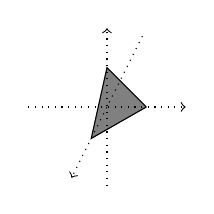
\begin{tikzpicture}[scale=.5]
				\draw[fill=gray] (1, 0)--(0, 1)--(-.4,  -.8)--(1, 0);
				\draw[->,  dotted] (-2, 0)--(2, 0); \draw[->,  dotted] (0, -2)--(0, 2) ; \draw[->,  dotted] (.9,  1.8)--(-.9,  -1.8) ;
			\end{tikzpicture}\\
\end{tabular}
\end{example}
Simplices have the property that their boundaries are created of smaller simplices. For instance,  a 2-simplex (triangle) has 3 boundary 1-simplices (edges.) A 3-simplex (tetrahedron) has 4 boundary 1-simplices. In general a $k$-simplex has $k+1$ boundary $k-1$-simplices,  called \textbf{facets}.\\
A simplex has more than just $k-1$ dimensional facets; it also has boundary components of dimension $k-l$. Each boundary component is uniquely specified by the $k-l+1$ corner vertices it uses. If we wanted to build more complicated spaces by gluing together simplices, one would imagine that we would take these simplices and join them together along boundary strata picked out by identifying their vertices.\\

\examplefigure{Here is an example of a topological space constructed from simplices. It uses 8 vertices, has 13 edges, 8 faces, and 1 3-simplex (the right simplex is not filled in.) Notice that this topological space doesn't have a consistent notion of ``dimension''-- the dimension varies from 1-3 dimensional depending on which part of the complex you look at.}
{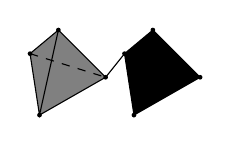
\begin{tikzpicture}[scale=.6]
			\draw[fill=gray](-.4,  -.8)-- (1, 0)--(0, 1)--(-.4,  -.8)--(-.6,  .5)--(0, 1);
			\draw[dashed](-.6, .5)--(1, 0);
		\fill (-.4, -.8)   circle[radius=.05] ;
		\fill (1, 0)   circle[radius=.05] ;
		\fill (-.6,  .5)   circle[radius=.05] ;
		\fill (0, 1)   circle[radius=.05] ;	
		\fill (1.6, -.8)   circle[radius=.05] ;
		\fill (3, 0)   circle[radius=.05] ;
		\fill (1.4,  .5)   circle[radius=.05] ;
		\fill (2, 1)   circle[radius=.05];
		\draw (1, 0)--(1.4,  .5);
		\draw[fill=\shadinga](1.6,  -.8)-- (3, 0)--(2, 1)--(1.6,  -.8)--(1.4,  .5)--(2, 1);
		\draw[dashed](1.4, .5)--(3, 0);
	 	\end{tikzpicture}}
In practice, it is simpler to build in this identification of simplices from the very beginning.   
\begin{definition}
	A \emph{finite abstract simplicial complex} is a pair $X=(\Delta, \mathcal S)$ where
	\begin{itemize}
	\item  $\mathcal S$ is a base set of vertices
	\item $\Delta\subset \mathcal P(S)$ is a finite set of \emph{simplices} 
	\end{itemize}
	where the simplices are downward closed. This means that whenever $\sigma\in \Delta$ and $\tau\subset \sigma$, then $\tau\in \Delta$. We say that $\sigma\in \Delta$ is a \emph{$k$-simplex} if $|\sigma|=k+1.$ The set of all $k$-simplices will be denoted $\Delta_k$. 
\end{definition}
\nomenclature{$\sigma$}{A simplex}
\nomenclature{$X=(\Delta, \mathcal S)$}{A simplicial complex}
These abstract simplicial complexes give us short and effective ways to describe topological spaces, and give us the same types of spaces as our gluing intuition (see Figure \ref{fig:simplicialcomplex} for an example. )
\begin{figure}
\centering
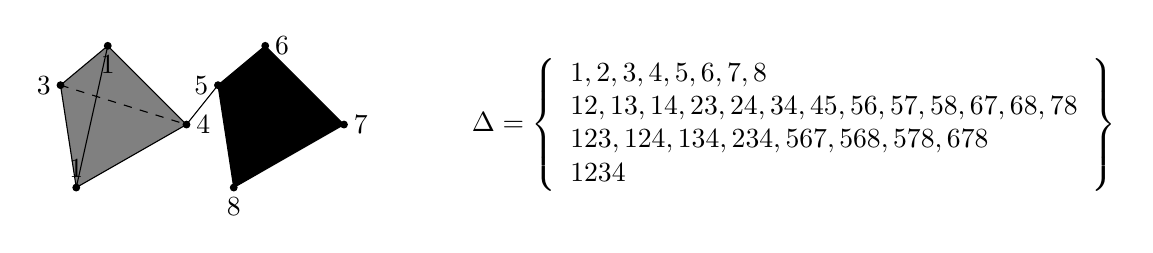
\begin{tikzpicture}
			\draw[fill=gray](-.4,  -.8)-- (1, 0)--(0, 1)--(-.4,  -.8)--(-.6,  .5)--(0, 1);
			\draw[dashed](-.6, .5)--(1, 0);
		\fill (-.4, -.8)   circle[radius=.05] node[above]{1};
		\fill (1, 0)   circle[radius=.05] node[right]{4};
		\fill (-.6,  .5)   circle[radius=.05] node[left]{3};
		\fill (0, 1)   circle[radius=.05] node[below]{1};	
		\fill (1.6, -.8)   circle[radius=.05] node[below]{8};
		\fill (3, 0)   circle[radius=.05] node[right]{7};
		\fill (1.4,  .5)   circle[radius=.05] node[left]{5};
		\fill (2, 1)   circle[radius=.05] node[right]{6};
		\draw (1, 0)--(1.4,  .5);
		\draw[fill=\shadinga](1.6,  -.8)-- (3, 0)--(2, 1)--(1.6,  -.8)--(1.4,  .5)--(2, 1);
		\draw[dashed](1.4, .5)--(3, 0);
\node[right] at (4.5,0) {$\Delta=\left\{\begin{array}{l}
	                	1, 2, 3, 4, 5, 6, 7, 8\\
	                	12, 13, 14, 23, 24, 34, 45, 56, 57, 58, 67, 68, 78\\
	                	123, 124, 134, 234, 567, 568, 578, 678\\
	                	1234
	                \end{array}\right\}$};
\end{tikzpicture}
\caption{A geometric representation of an abstract simplicial complex.}
\label{fig:simplicialcomplex}
\end{figure}
We usually denote a simplicial complex $\Delta$ and forego the set $S$, and sometimes we will only give the \emph{top dimensional simplices} of a simplicial complex when defining it. \\
Here are a few abstract simplicial complexes.
\begin{example}A \emph{graph} is a simplicial complex with the property that $|X|\leq 2$ for $X\in \Delta$. The elements of size 2 are called edges, and the elements of size 1 are called vertices. Similarly, the triangulated surfaces that we constructed before are examples of simplicial 2-complexes. 
\end{example}
\examplefigure[Disk]{
If $\mathcal S=\{1, \ldots, n+1\}$, then letting $\Delta=\mathcal P(\mathcal S)$ gives us a simplicial complex. This simplicial complex has one maximal $n$-simplex. When we want to refer to this simplicial complex, we will usually use the notation $D^n$, for the \emph{$n$-disk}.\\
Notice that there is a natural copy of $D_x^{n-1}\subset  D^n$, which is the disk consisting of all simplices except the last simplex $x$.   \label{exam:disk}}{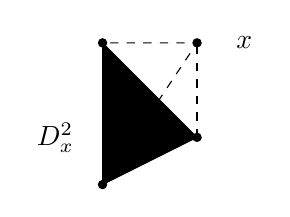
\begin{tikzpicture}[scale=.6]
\fill(-3,1) circle[radius=.1];
\fill(-1,1) circle[radius=.1];
\fill(-1,-1) circle[radius=.1];
\fill(-3,-2) circle[radius=.1];
\draw[fill=\shadinga] (-3,1) -- (-3,-2) -- (-1,-1) -- cycle;
\draw[dashed] (-3,-2) -- (-1,1) -- (-3,1);
\draw[dashed] (-1,-1) -- (-1,1);
\node at (0,1) {$x$};
\node at (-4,-1) {$D^2_x$};
\end{tikzpicture}}
\nomenclature{$D^n$}{The $n$-dimensional disk.}
A good intuition for a topological space is something akin to a ``wire frame'' model for a space. A growing area of applied mathematics looks at how we can associate ``good'' simplicial complexes to point-clouds which are suppose to represent some topological object. 

\examplefigure[Vietoris-Rips]{
  Given some subset $V$ of a metric space $M, \delta$, define the $L$ \emph{Vietoris-Rips complex} as the set of subsets of $V$ which have diameter less than $L$. The structure of the Vietoris-Rips complex is an active field of research in applied mathematics, image sensing, and communications.\project \label{proj:persistenthomology} The resulting topologies can be captured using a tool called \emph{persistent homology}. }{\includegraphics[scale=1]{simp_pershomo}}
 Sometimes we can create simplicial complexes without using topological intuition. Usually in these cases, we start with some other mathematical object, and associate to it a topological space. 
\begin{example} Let $\mathcal S$ represent the set of all possible edges on $n$ vertices. Notice that subsets $G\subset \mathcal S$ correspond to graphs. Define the chromatic complex $X_k=(\Delta, S)$ where $G\in \Delta$ whenever $G$ is $k$-colorable. This gives us the structure of a simplicial complex, as whenever $H\subset G$ is a subgraph and $G$ is $k$-colorable, then $G$ is $k$-colorable. \\ The above example extends to a lot of different properties of graph. One could take planarity, surface embeddability, or any other variety of ``monotonic graph property.'' It turns out that studying the topological properties of these spaces gives us data on algorithms that try to detect these above properties.\project One interesting application of this approach is topological methods in \emph{evasiveness}.
\end{example}
\begin{figure}
\centering

\includegraphics[scale=1]{simp_evasive}

\caption{The simplicial complex of triangle-free graphs on $3$ vertices. It is a 3-cycle, with vertices and edges labeled by graphs. }
\end{figure}
\begin{example}
Let $(P, <)$ be any poset. A \emph{chain} on $P$ is a subset of the form 
\[\{x_1< x_2\cdots < x_k\}.\]
Let $\mathcal S=P$, and let $\Delta$ be the set of all chains coming from the partial order. This form a simplicial complex, called the associated simplicial complex to $P$. 
\end{example}



Given any simplicial complex, we have a \emph{geometric realization} of the complex. Choose $S$ with finite size, and consider the affine space $(\RR^+)^{|S|}$ with coordinates $\{e_i\}_{i\in S}$. Then to the simplicial complex $X=(\Delta, \mathcal S)$, we associate the topological space 
\[|X|:=\bigcup_{\sigma \in \Delta} \text{Conv}(\{e_i\}_{i\in \sigma})\]
 This is a topological space. We will avoid working with the geometric realization, because it is not very combinatorial. \\
 Simplicial complexes are broad class of topological space; in fact, the majority of topological spaces that you might study are built out of simplicial complexes. Here are a few interesting examples of topological spaces that one can build. 
\begin{example}[Higher Dimensional Spheres]
A \emph{$n$-sphere} is cut out from $\RR^{n+1}$ by the equation
\[\sum_{i=1}^{n+1} x_i^2=0.\]
For us, a good model for the $n$-sphere is the boundary of the $n+1$ simplex. As a simplicial space, we can describe by letting $\mathcal S=\{1,\ldots, n+2\} $, and defined the simplicial complex
\[S^{n+1}=\mathcal P(\mathcal S)\setminus\{\{1,\ldots, n+2\}\}\]
\nomenclature{$S^n$}{The $n$ dimensional sphere}.  \label{def:nsphere}
\end{example}
While simplicial complexes give us hands on descriptions of topological spaces, they have two features which makes them practically difficult to use in topology:
\begin{itemize}
\item What is a map between simplicial complexes?
\item What does it mean for 2 simplicial complexes to be the same?
\end{itemize}
We'll put off both of these questions until Section \ref{sec:simplicialmaps}, and even then our answer might be a little less than satisfactory. 
\subsection{Simplicial Homology}
The tools that we have been developing for graphs and surfaces similarly work well in simplicial complexes. 
\begin{definition}
Let $X$ be a simplicial complex. Define the \emph{simplicial chain complex} $(C_\bullet(X), \partial)$ to have:
\begin{itemize}
\item Chain groups $C_k(X)$ which are the $\Z_2$ vector spaces generated on a basis of the $k$-simplices of $X$. 
\item A boundary differential  $\partial_k: C_k(X)\to C_{k-1}(X)$ defined by it's values taken on the basis $\{\sigma\in \Delta\;|\;\dim(\sigma)=k\}$ 
\[\partial_k(\sigma)=\sum_{\substack{\tau\subset \sigma\\ |\sigma\setminus\tau|=1}} \tau.\]
\end{itemize}
\label{def:simplicialhomology}
\end{definition}
The simplicial chain complex is our first example of a full chain complex (see Definition \ref{def:chaincomplex}.) contains a lot of data; in fact, provided that we know what the basis given by simplices is, equivalent data to that of the simplicial complex itself. As before, the ``useful topological data'' of a simplicial complex comes from the form of it's \emph{homology groups,}
\[H_k(X):=\frac{\ker \partial_k}{\im \partial_{k+1}}.\]
Following our intuition from graph complexes and surface complexes, we call $\ker\partial_k$ and $\im\partial_{k+1}$ the space of \emph{cycles} and \emph{boundaries} respectively. (See Definition \ref{def:homologygroups} for a more detailed exposition on the algebraic construction of homology groups. )
\begin{example}
The graph complex (Definition \ref{def:graphcomplex}) and embedded graph complex for triangulated nets(Definition \ref{def:surfacecomplex}) are both examples of simplicial chain complexes associated to simplicial complexes. \\
In the language of triangulated nets, two cycles $c_1, c_2\in \ker(\partial_1)$ represent the same \emph{homology class} if they are the boundary of some common sub-surface.
\end{example}
\begin{example}[Homology of Disk] \label{exam:diskhomology}
Recall that the $n$-disk was the simplicial complex on $n+1$ vertices that had every subset of vertices a simplex. In this set-up,
\[C_k(D^n)=\Z_2\{\sigma\subset\{1, \ldots, n+1\}\}\]
We will show that the homology of the $n$-disk is 
\[ H_k(D^n)=\left\{\begin{array}{ll} \Z_2 & k=0\\ 0 & k\geq 1 \end{array} \right. . \]
We prove this by induction on the dimension of the disk.\\
As a base case, $D^0$ is a point, so we have that $C_0(D^0)=\Z_2$, and all other chain groups are empty; the claim trivially follows.\\
For the induction step, let us assume that the statements holds for $D_x^n\subset D^{n+1}.$ Then we have 2 kinds of simplices: those that contain $x$, and those which do not. Recall that the $k$-simplices of $D^{n+1}$ that contain $x$ are in bijection with then $k-1$ simplices of $D^n$, whenever $k\neq 0$.  \ref{exam:disk}
With this claim, we have that when $k\neq 0$. 
\[C_k(D^{n+1})\simeq C_k(D_x^{n})\oplus C_{k-1}(D_x^{n}).\]
We will now try to reinterpret the differential. Our original chain complex:
\[
\begin{tikzcd}
\cdots & C_k(D^{n+1}) \arrow{r}{\partial_k} & C_{k-1}(D^{n+1})& \cdots \arrow{r} & C_1(D^{n+1})  \arrow{r} & C_0(D^{n+1})
\end{tikzcd}\]
can be rewritten after this reinterpretation:
\[
\begin{tikzcd}[row sep = small] 
\;&  C_{k-1}(D_x^{n})\arrow{r}{\partial^a} \arrow{rdd}{\partial^b} &  C_{k-2}(D_x^{n}) \arrow{r}& \cdots \arrow{r} &  C_{0}(D_x^{n})\arrow{r}{\partial^a} \arrow{rdd}{\partial^b} &  \Z_2\{x\}\\
 \cdots & \oplus & \oplus &  & \oplus & \oplus  \\
&  C_k(D_x^{n})\arrow{r}{\partial^c} &  C_{k-1}(D_x^{n})\arrow{r}& \cdots \arrow{r} & C_1(D_x^{n})\arrow{r}{\partial^c} &  C_0(D_x^{n}) \\
\end{tikzcd}
\]
where the top row corresponds to simplices that do not contain the point $x$, and the bottom row corresponds to those simplices that do contain $x$. The arrows in this diagram tell us that 
\begin{itemize}
\item $(\partial^a)$: Simplices that do contain $x$ can have their boundary in simplices that do contain $x$. 
\item  $(\partial^b)$: Simplices that do contain $x$ can have their boundary in simplices that do not contain $x$. 
\item  $(\partial^c)$: Simplices that do not contain $x$ may only have in their boundary simplices that do not contain $x$. 
\end{itemize}
Notice that the maps $\partial^b$ are all isomorphisms. This means that outside of $C_0(D^{n+1}$, the kernel of $\partial=\partial^1+\partial^b+\partial^c$ restricted to the top row is empty. Similarly, there is no element in the bottom row which is not contained in $\im(\partial).$. As a result, 
\[H_k(D^{n+1})=0 \;\;\;\; k\neq 0.\]
An examination shows that the $Z_2{x}$ is in the kernel of $\partial_0$, and is not in the image of the boundary maps $\partial_1$. Therefore, the homology $H_0(D^{n+1})=\Z_2$ can be though of as generated by the equivalence class $[x]$. 
\end{example}
We will eventually develop the necessary homological algebra tools to generalize this kind of proof. Before we continue with the construction of these tools, let's try to give a geometric interpretation to these homology groups:
\begin{example}[Homology of the Sphere]
Recall that we had defined the $n$-sphere in Definition \ref{def:nsphere} to be a hollowed out version of $D^{n+1}$. The homology of the sphere gives us an interpretation to what $H^n(\Delta)$, as 
\[
H_k(S^n)=\left\{\begin{array}{ll} \Z_2 & k\in \{0, n\}\\ 0 & \text{otherwise}\end{array}\right. .\]
To prove this, notice that whenever $k\neq n, n+1$ we have 
\[C_k(S^{n})=C_k(D^{n+1}),\]
so it suffices to check the homology at the $n$th place. Exercise \ref{exer:homsphere} shows that 
\[\ker (\partial_{n}: C_n(S^{n})\to C_{n-1}(S^{n})\simeq \Z_2\] is 1-dimensional. 
\end{example}
One often used metaphor for homology groups count the $k$-dimensional holes in a topological space. The above example corroborates that interpretation. \\
More succinctly, one should think of an element of $\ker(\partial_k)$ as a borderless sub-simplicial complex that one constructs out of simplifies. An element $\im(\partial_{k+1})$ is a boundary of a $k+1$ sub-simplicial complex. One might say that a $k$-dimensional subcomplex $Y$ is a ``hole'' if there is no $k+1$-dimensional subcomplex $Z$ which fills it. Translating this back to the language of homology, the space of holes of $X$ is 
\[\{Y\subset X \;|\; \not \exists (Z\subset X) ; \partial(Z)=Y\}\]
This is exactly the same as the homology elements of $X$. 

\examplefigure[Higher Homology of Torus]{
Let's look at an example of a space, and try to use the above intuition for guessing what the homology of a space is. \\
The \emph{3 -torus} can be constructed by taking the quotient $T^3:=\RR^3/\Z^3.$ One way to visualize this to imagine a room where:  The Floor and Ceiling have been glued together; The West and East walls have been identified;The North and South walls have been identified. \\
One could take a line of string and tie it into a loop by passing it through the north and south walls. This loop represents a 1-dimensional subspace which is not the boundary of any 2-dimensional subspace; it therefore represents a class in homology. Similarly, the Floor-Ceiling loop and West-East loop represent different homology classes. With this data, we guess that 
\[H^1(T^3)=(Z_2)^3.\]
Similarly, one can find 3 tori which are not the boundary of 3-dimensional subspaces, and giving us 
\[H^2(T^3)=(\Z_2)^3.\]}{\includegraphics[scale=1]{simp_highertorus}}
\section{Constructions in Simplicial Complexes}
In this section, we will explore some topological constructions that we may apply to simplicial complexes, which will parallel some of the constructions in homological algebra. This relationship between homological algebra and simplicial complexes is truly the beautiful core of this branch of mathematics. While elegant, this theory is a bit of a pedagogical nightmare as one is either required to learn 2 branches of mathematics separately without motivation, or develop 2 branches of mathematics simultaneously. We take the second approach, with these notes referencing the relevant results in Appendix \ref{append:homologicalalgebra} as necessary.
\subsection{Maps and Cones}
\begin{elevator}
We define what maps between simplicial spaces are. Perhaps the most important takaway is the creation of a \emph{cone} of a map, which gives us a way to understand what the ``kernel'' or ``cokernel'' of a map between simplicial spaces should be. This opens up new ways for us to compute homology quickly. 
\end{elevator}
As a noted from above, this subsection runs roughly parallel to \ref{append:chaincomplexes} and \ref{append:chaincones}; I apologize to the reader who uses these notes simultaneously, as there may be a great deal of page flipping in the future. \\
The only structure that a simplicial complex $X$ has is the order relation on the simplices, which is determined by the base set $\mathcal S$ of vertices. 
\begin{definition}
Let $X_1=(\Delta_1, \mathcal S_1)$ and $X_2=(\Delta_2, \mathcal S_2)$ be two simplicial complexes.  A \emph{map of abstract simplicial complexes $f:X_1\to X_2$ } is a map $F: \mathcal S_1\to \mathcal S_2$ so that the image of simplices in $\Delta_1$ are simplices in $\Delta_2$. This means whenever 
\[\sigma = \{x_1, \ldots, x_k\}\in \Delta_1\]
we have that the induced map on simplices is also a simplex. 
\[F(\sigma)=\{F(x_1), \ldots, F(x_k)\}\in \Delta_2.\]
\end{definition}
\begin{example}
In Example \ref{exam:disk} we showed that $D^{n-1}\subset D^n, $ and this inclusion can be represented by a map $i:\{1, \ldots, n\}\into \{1, \ldots, n+1\}$. 
\end{example}
\examplefigure{A map of simplicial complexes need not send simplices to simplices of the same dimension. A trivial example of a simplicial map simply sends every simplex to a single point. Here is a map between two simplicial complexes: the sphere and a path with 3 vertices. Notice that many of the triangular faces are ``flattened'' to edges, and sometimes several faces are flattened to the same edge; additionally, several of the edges are mapped to vertices. }{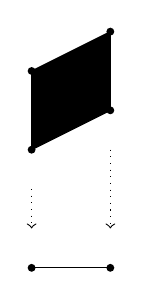
\begin{tikzpicture}[scale=.5]
\draw[fill=\shadinga] (-2,2) -- (-2,0) -- (0,1) -- cycle;
\draw[fill=\shadinga]  (-2,2) -- (0,3) -- (0,1);
\fill(-2,0) circle[radius=.1];
\fill(0,3) circle[radius=.1];
\fill(-2,2) circle[radius=.1];
\fill(0,1) circle[radius=.1];
\fill(0,-3) circle[radius=.1];
\fill(-2,-3) circle[radius=.1];
\draw (-2,-3) -- (0,-3) ;
\draw[dashed] (-2,0) -- (0,3);
\draw[->, dotted] (-2,-1) -- (-2,-2);
\draw[->, dotted] (0,0) -- (0,-2);
\end{tikzpicture}}
Maps of abstract simplicial complexes play well with the construction of the simplicial chain complex. 
\begin{claim}
Let $f: X\to Y$ be a map of simplicial complexes. Then we have an induced map of chain complexes $f_k: C_k(X)\to C_k(Y)$, which is chain map in the sense of Definition \ref{def:chainmap}.
\end{claim}
\begin{proof}
We need to give a definition of the induced maps on the chain complex, and also show that this satisfies the properties of being a chain map. We define the map $f_k:C_k(X)\to C_k(Y)$ by looking at its behavior on the basis $\{\sigma\}_{\sigma\in X,\dim(\sigma)=k}$ for $C_k(X)$. In this case, 
\[f_k(\sigma)= \left\{ \begin{array}{ll} F(\sigma) & \text{if $\dim F(\sigma)=k$}\\ 0 & \text{otherwise}\end{array}\right. \]
To show that this is a chain map, we need to prove that 
\[f_{k-1} \partial^{X}_k = \partial^{Y}_{k} f_k.\]
We can check this is true by checking on a basis: 
\begin{align*}
\partial^{Y}_{k} f_k(\sigma)=  \left\{ \begin{array}{ll} \partial^Y_k(f(\sigma) & \text{if $\dim f(\sigma)=k$}\\ 0 & \text{otherwise}\end{array}\right. \\
\end{align*}
In the first case, 
\begin{align*} \partial^Y_k(f(\sigma)= &\sum_{\substack{\tau\subset F(\sigma)\\ |\sigma\setminus\tau|=1}} \tau
\intertext{Since $F|_{\sigma}$ is a bijection, we have that for each such $\tau\subset \partial \sigma$, there is a $\tilde \tau\in \Delta_1$ so that $f_{k-1}(\tilde \tau)= \tau. $}
=& \sum_{\substack{\tau\subset f(\sigma)\\ |\sigma\setminus\tau|=1}} f(\tilde \tau)\\
=& f_{k-1}(\sum_{\substack{\tau\subset F(\sigma)\\ |\sigma\setminus\tau|=1}} (\tilde \tau)\\
=& f_{k-1}\partial_k(\sigma).
\end{align*}
In the second case, suppose that $f(\sigma)=0$. We now break into 2 cases:
\begin{itemize}
\item Suppose that $\dim F(\sigma)< \dim(\sigma-1)$. Then for every $\{\tau\subset F(\sigma)\;|\;|\sigma\setminus\tau|=1\}$ we have that $f(\tau)=0$. Then 
\[f_{k-1} \partial_k (\sigma)=0. \]
\item Suppose that $\dim F(\sigma)=\dim(\sigma-1)$. Then label the vertices of $\sigma=\{x_1, \ldots, x_{k+1}\}$. We may assume that $F(x_1)=F(x_2)$. Let $\tau_1=\sigma\setminus \{x_1\}$, and $\tau_2=\sigma\setminus\{x_2\}$. We now break the boundary into 3 different terms:
\begin{align*}
f_{k-1} \partial_k (\sigma) =&f_{k-1}\left( \sum_{\substack{\tau\subset \sigma\\ |\sigma\setminus\tau|=1}} \tau\right)\\
=& f_{k-1} \left( \left(\sum_{\substack{\tau\subset \sigma\\ |\sigma\setminus\tau|=1\\ \{x_1,x_2\}\subset \tau }} \tau \right)+\tau_1+\tau_2 \right)\\
\intertext{Notice that $\dim(F(\tau))\neq \dim \tau$ whenever $\{x_1, x_2 \} \subset \tau.$. }
=& f_{k-1} (\tau_1+\tau_2)
\intertext{Furthermore, $f_{k-1}(\tau_1)=f_{k-1}(\tau_2).$ Since we work in $\Z_2$,}
=& 0
\end{align*}
\end{itemize}

\end{proof}
Whenever we have a map of simplicial complexes, we can construct a new simplicial complex called the \emph{cone} of that map. 
\begin{definition}
Let $X$ and $Y$ be simplicial complexes. Let $f:X\to Y$ be a map of simplicial complexes. Then the \emph{cone} of $f$ is the simplicial complex $\cone(f)$ with
\begin{itemize}
\item Base set $\mathcal S(\cone(f)) = \mathcal S(Y)\cup\{x_0\}$.The extra vertex $x_0$ is called the \emph{cone point.}
\item Simplifies given by $\Delta(\cone(f))= \Delta(Y)\cup\{ F(\sigma)\cup\{x_0\} \}_{\sigma\in \Delta(X)}$. 
\end{itemize}
\end{definition}
The intuition behind a map $X\to Y$ is to image the following process: Take $Y\subset X$ as a subcomplex given by an inclusion. Then extrude $Y$ out of $X$ to get a top-hat like figure. Finally, contract the top of this extruded figure to a point, creating a shape which is a bit like a wizard's cap. See Figure \ref{fig:cone} for a drawing of the general process. 
\begin{figure}
\centering
\includegraphics[scale=1]{simp_makeacone}
\caption{The process to make a cone: first extrude, then pinch.}
\label{fig:cone}
\end{figure}


\examplefigure[Cone of Identity]{ Let $X$ be any simplicial complex, and look at the map $\id: X\to X$. Then $\cone(\id)$ is the pyramid created by taking $X$ to be the base. Notice that the resulting shape is always contractible. We will later show that the homology of such cones is always trivial. One particular case of interest is the disk. In this case, notice that $\cone(\id:D^n\to D^n)=D^{n+1}$. The decomposition of simplices into 2 types, as in Example \ref{exam:disk} comes from this construction. \label{exam:identitycone} }{\includegraphics[scale=1]{simp_coneid}}

\examplefigure[Constructing Spheres]{ Let $D^n$ be the $n$ dimensional disk, and let $S^{n-1}$ be the $n-1$ dimensional sphere. There is a natural inclusion $i: S^{n-1}\into D^n$, where the sphere is mapped to the boundary of the disk. The cone of this map is $S^n$. One can visualize this by thinking of $D^n$ as a sheet of cloth, $S^{n-1}$ as the boundary of that cloth, and the cone operation as making a ``knapsack'' by tieing together the edges. \label{exam:conesphere}}{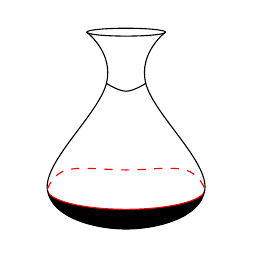
\begin{tikzpicture}[scale=.5]

\fill[\shadinga]  plot[smooth, tension=.7] coordinates {(0,2) (0.5,0.7) (-1,-2) (1,-3) (3,-2) (1.5,0.7) (2,2)};
\draw[red, fill=white] (1,-2) ellipse (2 and 0.5);
\fill[white]  (-1.5,2) rectangle (4,-2);
\draw  plot[smooth, tension=.7] coordinates {(0,2) (0.5,0.7) (-1,-2) (1,-3) (3,-2) (1.5,0.7) (2,2)};
\draw  plot[smooth, tension=.7] coordinates {(0.5,0.7) (1,0.5) (1.5,0.7)};
\draw[dashed, red]  plot[smooth, tension=.7] coordinates {(-1,-2) (-0.5,-1.5) (1,-1.5) (2.5,-1.5) (3,-2)};
\draw  (1,2) ellipse (1 and 0.1);
\end{tikzpicture}}

\subsubsection{Cones: An Important Philosophical Digression}
What do cones really mean? Perhaps the most important philosophy that we can take away from the cone construction is that topological spaces come with some notion of what a kernel or cokernel is!\\
Let's analyze in details the ways that cones mgive us kernels and cokernels. Let's suppose that $X\subset Y$ is some subspace, and let $\cone$ be the cone of the inclusion map from $f: X\into Y$.  Then $X, Y,$ and $\cone$ all have interpretations of kernels and cokernels. We're going to have 6 different cases to look at here, so hang on!

\noindent \textbf{Exactness at the $Y$:} Let's first look at the three maps 
\[X \xrightarrow{f} Y \xrightarrow{i} \cone.\]
Let's start with the example of a disk being included into the cone.
\[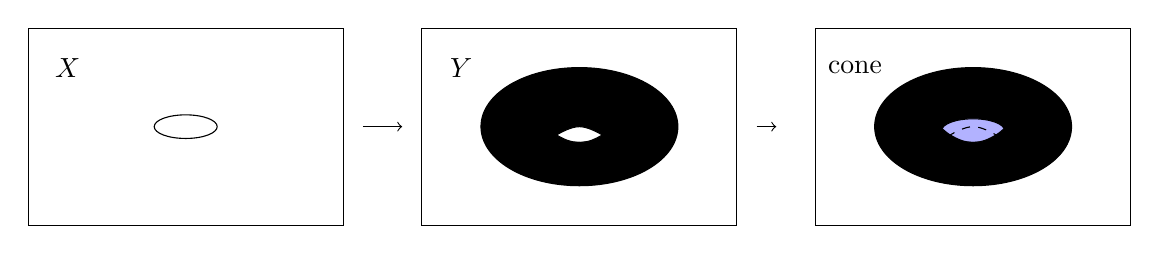
\begin{tikzpicture}[scale=.5]\draw[fill=\shadinga]  plot[smooth cycle, tension=1] coordinates {(-3,4) (-5.5,2.5) (-3,1) (-0.5,2.5)};
\begin{scope}
\clip  plot[smooth, tension=.7] coordinates {(-4,2.7) (-3.6,2.3) (-3,2.1) (-2.4,2.3) (-2,2.7)};
\draw[fill=white]  plot[smooth, tension=.7] coordinates {(-4,2) (-3,2.5) (-2,2)};
\draw  (-3,2.4) ellipse (.8 and 0.3);
\end{scope}
\draw[dotted]  (-3,2.4) ellipse (.8 and 0.3);
\draw  plot[smooth, tension=.7] coordinates {(-4,2.7) (-3.6,2.3) (-3,2.1) (-2.4,2.3) (-2,2.7)};
%\draw  plot[smooth cycle, tension=.7] coordinates {(-2.5,3) (-4,3.5) (-4.5,2.5) (-3.5,1.5) (-2,1.5) (-1,2) (-1.5,3)};
\draw[fill=\shadinga]  plot[smooth cycle, tension=1] coordinates {(7,4) (4.5,2.5) (7,1) (9.5,2.5)};
\begin{scope}[shift={(10,0)}]
\clip  plot[smooth, tension=0.7] coordinates {(-4,2.7) (-3.6,2.3) (-3,2.1) (-2.4,2.3) (-2,2.7)};
\draw[fill=blue!30]  (-3,2.4) ellipse (.8 and 0.3);
\draw[dashed]  plot[smooth, tension=0.7] coordinates {(-4,2) (-3,2.5) (-2,2)};
\end{scope}
\draw  plot[smooth, tension=.7] coordinates {(6,2.7) (6.4,2.3) (7,2.1) (7.6,2.3) (8,2.7)};
%\draw  plot[smooth cycle, tension=.7] coordinates {(7.5,3) (6,3.5) (5.5,2.5) (6.5,1.5) (8,1.5) (9,2) (8.5,3)};
\draw  (-13,2.5) ellipse (.8 and 0.3);
\draw  (-7,5) rectangle (1,0);
\draw  (3,5) rectangle (11,0);
\draw  (-9,0) rectangle (-17,5);
\node at (-16,4) {$X$};
\node at (-6,4) {$Y$};
\node at (4,4) {cone};
\draw[->] (-8.5,2.5) -- (-7.5,2.5);
\draw[->] (1.5,2.5) -- (2,2.5);
\end{tikzpicture}\]
In this sequence, we want to say that

\textfigure[9cm]{\textbf{ $X$ is like a kernel} for the map \[i: Y\to  \cone.\] This piece of the picture is the easiest to see. Suppose that $\alpha\in H_k(Y)$ is a homology class in $Y$. However, suppose that $i(\alpha)$ has a filling in $\cone$. Then it must be the case that $\alpha$ is filled in by the ``coney part'' of $\cone$, and it follows that $\alpha$ comes from a class $\beta\in H_k(X)$. Since every homology class in $\ker(i: Y\to \cone)$ is represented by some homology class of $X$, we get that $X$ is a good topological representative for the kernel. }{
\includegraphics[scale=1]{simp_les1}}
\textfigure[9cm]{ Now, we would like to show that $\cone$ is the cokernel for the map $f:X\to Y$. Suppose that $\alpha\in H_k(Y)$ is one that comes from  $H_k(X)$. Then in the cone, $\alpha$ has a filling, so $i(\alpha)=0$. Similarly, one can show that homology classes $\beta$ of $Y$ which do not come from $X$ survive in the cone. $H_k(\cone) $ now represents homology classes $H_k(Y)$ not arrising from $H_k(X)$, which can be restated as saying that $\cone$ is the cokernel of $Y\to X$. }{\includegraphics[scale=1]{simp_les2}}
\begin{enumerate}
\item Now let's look at the three maps 
\[Y \xrightarrow{i} \cone \xrightarrow{\pi} X[-1].\]
Here the map $\pi$ is the ``cone chopping'' map, which take homology classes of $\cone$ and transfers them to homology classes of $X$ by first chopping off the top and brim of the cone, and then squishing them down. Notice that this drops the dimension of the homology class by 1 (due to the squishing.)
\[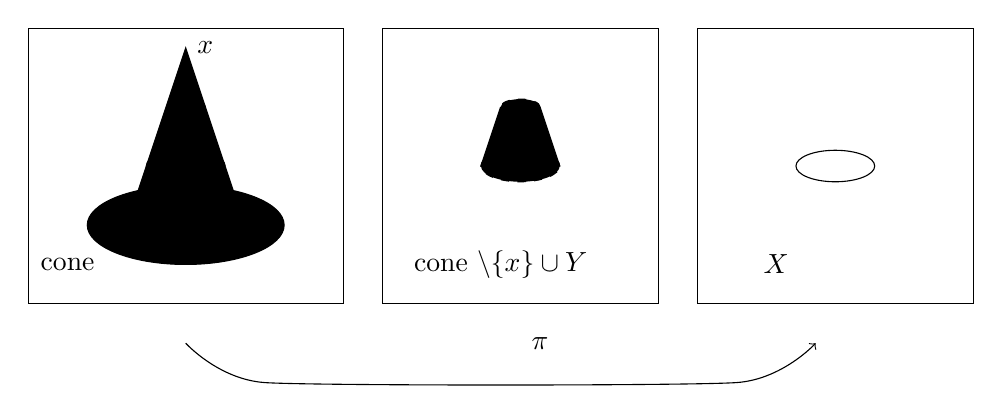
\begin{tikzpicture}[scale=.5]
\draw[fill=\shadinga]  (8,0) ellipse (2.5 and 1);
\draw[fill=\shadinga]  (8,0) ellipse (1.5 and 0.5);
\draw[fill=\shadinga] (6.5,0) -- (8,4.5) -- (9.5,0);
\draw[dashed]  (8,3) ellipse (0.5 and .2);
\draw[dashed]  (8,1.5) ellipse (1 and .4);
\node at (8.5,4.5) {$x$};
\draw[fill=\shadinga] (16,3) -- (15.5,1.5) -- (17.5,1.5)--(17,3);
\draw[dashed, fill=\shadinga]  (16.5,3) ellipse (0.5 and .2);
\draw[dashed, fill=\shadinga]  (16.5,1.5) ellipse (1 and .4);
\draw[->] (16.2,2.6) -- (16,1.6);
\draw[->] (16.8,2.6) -- (17,1.6);
\draw[->] (16.5,2.5) -- (16.5,1.5);
\draw  (24.5,1.5) ellipse (1 and .4);
\draw  (4,5) rectangle (12,-2);
\draw  (13,5) rectangle (20,-2);
\draw  (21,5) rectangle (28,-2);
\node at (5,-1) {cone};
\node at (16,-1) {cone $\setminus \{x\}\cup Y$};
\node at (23,-1) {$X$};
\draw[->]  plot[smooth, tension=.3] coordinates {(8,-3) (10,-4) (22,-4) (24,-3)};
\node at (17,-3) {$\pi$};
\end{tikzpicture}\]
\begin{itemize}
\item Let's reason why $Y$ is like a kernel for $\pi$. Let's suppose that there is a homology class $\alpha\in H_k(\cone)$ which is in the kernel of $\pi$.  One might reason that this means there is a way to take that homology class and move it off of the cone point. We could then deform $\alpha$ so it lies in the brim of the one, and therefore comes from a class in $Y$. Under this line of reasoning, $Y$ represents $\ker \pi$.
\[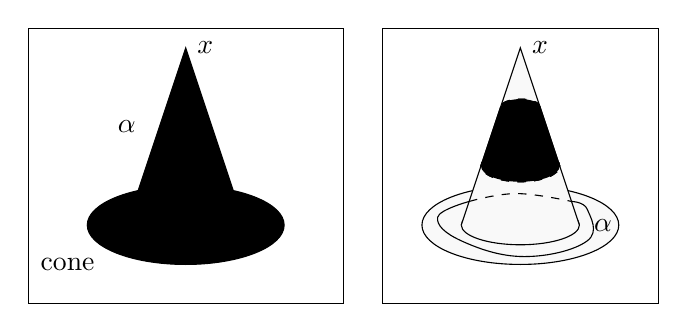
\begin{tikzpicture}[scale=.5]
\draw[fill=\shadinga]  (8,0) ellipse (2.5 and 1);
\draw[fill=\shadinga]  (8,0) ellipse (1.5 and 0.5);
\draw[fill=\shadinga] (6.5,0) -- (8,4.5) -- (9.5,0);
\node at (8.5,4.5) {$x$};
\draw[fill=gray!05]  (16.5,0) ellipse (2.5 and 1);
\draw[fill=gray!5]  (16.5,0) ellipse (1.5 and 0.5);
\draw[fill=gray!5] (15,0) -- (16.5,4.5) -- (18,0);
\draw[dashed]  (16.5,3) ellipse (0.5 and .2);
\draw[dashed]  (16.5,1.5) ellipse (1 and .4);
\node at (17,4.5) {$x$};
\draw[fill=\shadinga] (16,3) -- (15.5,1.5) -- (17.5,1.5)--(17,3);
\draw[dashed, fill=\shadinga]  (16.5,3) ellipse (0.5 and .2);
\draw[dashed, fill=\shadinga]  (16.5,1.5) ellipse (1 and .4);
\draw[->] (7.7,1.6) -- (7,0);
\draw[->] (8.6,1.2) -- (9,0);
\draw[->] (8.2,1.4) -- (8,0);
\draw  (4,5) rectangle (12,-2);
\draw  (13,5) rectangle (20,-2);
\node at (5,-1) {cone};
\draw  plot[smooth, tension=.7] coordinates {(7.4,2.6) (7.4,1.8) (8.2,1.6) (9,1.5)};
\draw[dashed]  plot[smooth, tension=.7] coordinates {(7.4,2.6) (8.2,2.4) (9,1.5)};
\node at (6.5,2.5) {$\alpha$};
\draw  plot[smooth, tension=.7] coordinates {(15.2,0.6) (14.4,0.2) (15,-0.4) (16.6,-0.8) (18.2,-0.4) (18.2,0.4) (17.8,0.6)};
\draw[dashed]  plot[smooth, tension=.7] coordinates {(15.2,0.6) (16.4,0.8) (17.8,0.6)};
\node at (18.6,0) {$\alpha$};
\end{tikzpicture}\]
\item The homology classes of $\cone$ come in two types: those which go through the cone point, and those which come directely from $Y$. This decomposition of the cone suggests that the cokernel of $i: Y\to \cone$ is exactly the homology classes which survive the cone chopping map. 
\end{itemize}
\item Finally, there is the sequence of maps 
\[\cone[1] \xrightarrow{\pi} X\xrightarrow{i} Y\]
\begin{itemize}
\item Let's bring our focus on why $\cone$ is suppose to be a kernel of $i: X\to Y$. Suppose that a homology class $\alpha\in H_k(X)$ has a filling in $Y$, so $f(\alpha)=0$. Let $\beta\in H_{k+1}(Y)$ be a choice of filling so that $\partial(\beta)=\alpha$.  Then imagine we make a knapsack out of $\beta$ ala Example \ref{exam:conesphere}. This gives us a new homology class $\tilde \beta$ in $B$, with $\pi(\beta)=\alpha$. This ``knapsack'' construction allows us to represent elements in the kernel of $f: X\to Y$ by elements of one dimension higher in the cone.
\[\includegraphics[scale=1]{simp_coneknapsack}\] 
\item Finally, which elements of $\alpha\in H_k(X)$ are not represented by the image of the neck-cutting map $\pi: X\to Y$. These are the elements which are not built by knapsacks; therefore, they are elements of $X$ which do not admit fillings in both the point and brim of the cone. Therefore, $ \alpha$ admits no filling in $Y$, so it is represented by a homology class $f(a)\in H_k(Y)$, making $Y$ the cokernel. 
\end{itemize}
\end{enumerate}

\subsubsection{Back to the Mathematics}
The cone construction is useful not only because it gives us a quick way to construct new topological spaces, but because it allows us to compute the homology of those new spaces quickly. The construction of cones carries over well to homological algebra in the form of the cone of a map between chain complexes, see Definition \ref{def:chaincone}.
\begin{claim}
Let $f: X\into Y$ be an injective map of simplicial complexes.  Then the simplicial chain complex of the cone is related to the cone of the simplicial complexes, in that:
\[C_\bullet(\cone(f: X\to Y))= \cone_\bullet(f:C_\bullet(X)\to C_\bullet(Y)) \oplus \Z_2\]
More specifically, whenever $k\neq 0,$
\[C_k(\cone(f: X\to Y)) = C_{k-1}(X)\oplus C_k(Y)\]
and when $k=0$, 
\[C_k(\cone(f:X\to Y)=C_0(Y)\oplus \Z_2.\]
The differential is given by the matrix
\[
\partial_k^{cone}=\begin{pmatrix} -\partial^X_{k-1}&0\\ f_{k-1} & \partial_{k}^X \end{pmatrix}
\]
whenever $k\neq 0$. 
\end{claim}
\begin{proof}
We check in two steps: first we will show that the chain groups match up, and then we will show that the differential agrees.\\
To show that the chain groups match up, we simply need to observe that whenever $f:X\into Y$ is an injective map, and $k\neq 0$
\[\Delta_k(\cone(f))=\Delta_{k-1}(X)\sqcup \Delta_{k}(Y).\]
As disjoint union becomes direct sum:
\[C_k(\cone(f: X\to Y)) = C_{k-1}(X)\oplus C_k(Y).\]
In the case that $k=0$, we need to add an additional simplex, $\{x\}$, contributing to the extra term that shows up. \\
For the differential, we look at $\partial_k^{\cone(f)}$ with it's domain restricted to either $C_{k-1}(X)$ or $C_k(Y)$. 
\begin{itemize}
\item If we restrict the domain to $C_{k}(Y)$, this corresponds to looking at boundaries of simplices that do not contain the vertex $x$. As a boundary of a simplex that does not contain $x$ will not contain $x$ itself, we have that $\im \partial^{\cone(f)}_{k}|_{C_k(Y)}\subset C_{k-1}(Y)$, and is the usual boundary map on $Y$. 
\item If we restrict the domain to $C_{k-1}(X)$, this corresponds to looking at the boundaries of simplices that contain the vertex $x$. Let $\sigma$ be such a simplex. Then $\partial_{k}^{\cone(f)}(\sigma)$ has 2 kinds of boundary components:
\begin{itemize}
\item The boundary components that do contain $x$. In this case, we may re-identify them with elements of $C_{k-2}(X)$, and as a result, we have that a portion of the boundary map $\partial_{k}^{\cone(f)}|_{C_{k-1}(X)}$ corresponds to simplices in $C_{k-2}(X)$. The restriction of the map to this domain and codomain\footnote{You'll notice here that we've inserted a $-$ sign. If we were working with orientations, this would be necessary. However, in our case, it is notationally convenient (as it matches our definition of cones from homological algebra,) and costs us nothing (as we work mod 2. )} is $-\partial_{k-1}^X$. 
\item Let us now look at the boundary components of $\sigma$ which do not contain $x$. These will be simplices in $C_{k-1}(Y)$, and this identification is given by the map $f$ which is used to construct the cone. 
\end{itemize}
\end{itemize}
We can assemble this datum into a single diagram 
\[
\begin{tikzcd}[row sep = small] 
\;&  C_{k-1}(X)\arrow{r}{-\partial^X_{k-1}} \arrow{rdd}{f_{k-1}} &  C_{k-2}(X) \arrow{r}& \cdots \arrow{r} &  C_{0}(X)\arrow{r}{-\partial^X_0} \arrow{rdd}{f_0} &  \Z_2\{x\}\\
 \cdots & \oplus & \oplus &  & \oplus & \oplus  \\
&  C_k(Y)\arrow{r}{\partial^Y_k} &  C_{k-1}(Y)\arrow{r}& \cdots \arrow{r} & C_1(Y)\arrow{r}{\partial^Y_1} &  C_0(Y) \\
\end{tikzcd}.
\]
Converting the diagram into the form of a matrix:
\[
\partial_k^{cone}=\begin{pmatrix} -\partial^X_{k-1}&0\\ f_{k-1} & \partial_{k}^X \end{pmatrix}
\]
whenever $k\neq 0$. 
\end{proof}
\begin{remark}
One may notice that there is a large inconvenience caused by the existence of an additional $\Z_2$ which one must insert into the degree $0$ chain group. One way to work around this is to work with \emph{reduced homology theory}, where every space $X=(\Delta, \mathcal S)$ is thought of having an additional component in degree $-1$ corresponding to the empty set of the simplicial complex. One could then redefine the chain groups to be the 
\[\tilde C_k(X):= \left\{\begin{array}{ll} C_k(X) & k\neq -1\\ \Z_2 & k= -1\end{array}\right.\]
where the differential is inherited from the regular chain complex. \\
While the only difference between homology and reduced homology that $\dim H_0(X)= \dim \tilde H_0(X)+1$, this small price allows you to make the statement 
\[\tilde C_\bullet(\cone(f:X\to Y))= \cone_\bullet(f: \tilde C_\bullet(X)\to \tilde C_\bullet(Y)).\]
However, as the idea of a $-1$ dimensional simplex is somewhat awkward for the purposes of drawing pictures and intuition otherwise, we've eliminated them from this book outside of this remark. 
\end{remark}
With this new construction, we can bring the tools of homological algebra to bear on the problems of topological spaces. In Theorem \ref{thm:leqfromcone}, we prove that whenever $h_\bullet:A_\bullet\to B_\bullet$ is a chain map, then we have the following long exact sequence (See Definition \ref{def:exactsequence}) of homology groups:
\[\begin{tikzcd}
\cdots \arrow{r}{h_*} & H_k(B)\arrow{r}{i_*} & H_k(\cone(h)) \arrow{r}{\pi_*} &  H_k(A[-1]) \arrow{r}{h_*}  & H_{k-1}(B) \arrow{r} & \cdots
\end{tikzcd}.\]
As expected, this result carries over into homological algebra. 
\begin{corollary} \label{cor:coneles}
Suppose that $f: X\to Y$ is an injective map of simplicial spaces. Then there is a long exact sequence :
\[\begin{tikzcd}
\cdots \arrow{r}{f_*} & H_k(Y)\arrow{r}{i_*} & H_k(\cone(h)) \arrow{r}{\pi_*} &  H_{k-1}(X) \arrow{r}{h_*}  & H_{k-1}(Y) \arrow{r} & \cdots 
\end{tikzcd}\]
which terminates 
\[\begin{tikzcd}
\cdots \arrow{r}{f_*} & H_0(Y)\arrow{r}{i_*} & H_0(\cone(h)) \arrow{r}{\pi_*} &  \Z_2
\end{tikzcd}.\]
\end{corollary}
We can use this technique to greatly shorten our proof of Example \ref{exam:diskhomology}. 
\begin{claim}
Let $\id_X: X\to X$ be the identity. Then $\cone(\id_X)$ has trivial homology except in degree $0$. (See Example \ref{exam:identitycone}.)
\end{claim}
\begin{proof}
From Corollary $\ref{cor:coneles}$ we can build the long exact sequence 
\[\begin{tikzcd}
\cdots\arrow{r}& H_k(X) \arrow{r}{\id_*} & H_k(X)\arrow{r}{i_*} & H_k(\cone(h)) \arrow{r}{\pi_*} &  H_{k-1}(X) \arrow{r}{\id_*}  & H_{k-1}(X) \arrow{r} & \cdots 
\end{tikzcd}\]
whenever $k\neq 0$. By applying the Rank-Nullity Theorem, 
\[H_k(X)(\cone(h))\simeq \ker(\pi_*)\oplus \im(\pi_*). \]
Since this sequence is exact, 
\[H_k(X)(\cone(h))\simeq \im(i_*)\oplus \ker(\id_*). \]
The identity map is injective, so $\ker(\id_*)=0$. To compute the image of $i_*$, we use Rank-Nullity and exactness again,
\[H_k(X)\simeq \ker(i_*)\oplus \im(i_*) \simeq \im(\id_*)\oplus \im(i_*).\]
As $\id_*$ is surjective, we similarly conclude that $\im(i_*)=0$. Putting this together, 
\[H_k(X)(\cone(h))\simeq \im(i_*)\oplus \ker(\id_*)=0. \]
In the case where $k=0$, the long exact sequence
\[\begin{tikzcd}
\cdots \arrow{r}{f_*} & H_0(Y)\arrow{r}{i_*} & H_0(\cone(h)) \arrow{r}{\pi_*} &  \Z_2
\end{tikzcd}\]
allows us to conclude that $H_0(\cone(\id))=\Z_2.$
\end{proof}


\section{Mayer-Vietoris Sequence}
We finally return to one of the core concepts of this course: given a decomposition of a space $X=A\cup B$, what can we tell about the topology of $X$ in terms of the topology of $A$ and $B$? 
\begin{definition}
Let $X$ be a topological space. The \emph{$k$th Betti number} is the dimension of the homology group 
\[b_k(X):=\dim H_k(X). \]
\end{definition}
While the Betti numbers $b_{k>0}$ have many interpretations, the $0$th Betti number simply counts the number of connected components. 
\begin{claim}
Let $X$ be a topological space. Then $b_0(X)$ is the number of connected components of $X$. 
\end{claim}
At the start of the course, we alluded that we would like an algorithm to compute the number $b_0(X)$ via an inclusion-exclusion principle on a decomposition of $X$ into smaller topological spaces. Let's look at an example where this works, and an example that shows that our theory requires some more depth. 
\begin{example}
Let $X$ be a collection of points, so we have no higher dimensional simplices. Then $b_0(X)$ counts the number of points in $X$, and clearly we that $X$ should respect the principle of inclusion-exlusion. 
\end{example}
\examplefigure{Let $S^1=A\cup B$ as drawn in the figure. Let's try to compute the number of connected components of $S^1$ using this decomposition. $A\cap B$ has two connected components, so we would have that 
\[b_0(A)+b_0(B)-b_0(A\cap B)=0\]
which means that we cannot use the principle of inclusion-exclusion to compute the number of connected components of the circle. The obstruction in this case to the principle of inclusion-exclusion working is the presence of nontrivial homology in $H_1(S^1)$.  }{\includegraphics[scale=1]{simp_incexc}}

While we cannot use the principle of inclusion-exclusion to compute the number connected components, we can get an inclusion-exclusion like principle to work homologically. For full details on how to generalize inclusion-exclusion like principles to general settings, see Appendinx \ref{append:inexzigzag}.
\begin{theorem}[Mayer-Vietoris]
Let $A, B, X$ be topological space. Let 
\begin{align*} j_A:A\to& X\\
j_B: B\to& X
\end{align*}
 be two inclusions of topological spaces so that $A\cup B=X$. Let $A\cap B$ be the common intersecion of $A$ and $B$ in $X$, with the natural inclusions 
 \begin{align*}
 i_A:A\cap B\to& A \\
  i_B: A \cap B\to & B
 \end{align*}
 Then there is a short exact sequence of chain complexes
 \[\begin{tikzcd}[row sep=tiny]
  \;& & C_\bullet(A) \arrow{dr}{j_A}\\
 0 \arrow{r}& C_\bullet(A\cap B)\arrow{ru}{i_A} \arrow{rd}{i_B} & \oplus & C_\bullet(X)\arrow{r} & 0\\
 & & C_\bullet(B) \arrow{ur}{-j_B}
 \end{tikzcd}\]
 This in turn gives us a long exact sequence on homology from Lemma \ref{lemma:zigzag}.
 \[\cdots\to  H_{k+1}(X)\to H_k(A\cap B)\to H_k(A)\oplus H_k(B)\to H_k(X)\to H_{k-1} (A\cap B)\to \cdots \]
\end{theorem}
\begin{proof}
To show that this is an exact sequence, we need to check that the chain maps form exact sequences of vector spaces at each grading $k$:
\[\begin{tikzcd}
0 \arrow{r} C_k(A)\arrow{r}{i_A\oplus A_B} & C_k(A)\oplus C_k(B) \arrow{r}{j_A\oplus (-j_B)} & C_k(X)\arrow{r} & 0.
\end{tikzcd}\]
Let's start by checking exactness at the first position of the sequence. 
\[
\begin{tikzcd}
0 \arrow{r} C_k(A)\arrow{r}{i_A\oplus A_B} & C_k(A)\oplus C_k(B)
\end{tikzcd}\]
The statement of exactness at this point is that $\ker (i_A\oplus A_B)=0$, or that the map is injective. Since both $i_A$ and $i_B$ are injective on simplices, their induced maps are injective on the chain complexes. The direct sum of injective maps along the domain is again injective, so we exactness at the first place. \\
At the last position of the sequence, 
\[
\begin{tikzcd}
C_k(A)\oplus C_k(B) \arrow{r}{j_A\oplus(- j_B)} & C_k(X)\arrow{r} & 0
\end{tikzcd}\]
exactness means that $\im{j_A\oplus j_B}=C_k(X)$, or that this map is surjective. Since every simplex of $X$ is one coming from $A$ and or $B$, we have that the map surjects on simplices, and therefore on chain complexes as well. \\
The only tricky part of the argument is on the middle section, 
\[ \begin{tikzcd} C_k(A)\arrow{r}{i_A\oplus A_B} & C_k(A)\oplus C_k(B) \arrow{r}{j_A\oplus(- j_B)} & C_k(X)\end{tikzcd}\]
Here, the statement is that $\ker(j_A\oplus(- j_B))=\im (i_A\oplus A_B). $ The kernel of the map $(j_A\oplus(- j_B))$ consists exactly of pairs $(a,b)$ where $j_A(a)=j_B(b)$. Since every such element comes from a chain in $A\cap B$, we have that this is the image of $i_A\oplus i_B$. \\
Once we know that the short seqeunce of chain complexes is exact, the long exact sequence of homology groups
 \[\cdots\to  H_{k+1}(X)\to H_k(A\cap B)\to H_k(A)\oplus H_k(B)\to H_k(X)\to H_{k-1} (A\cap B)\to \cdots \]
 follows from the application of the Zig-Zag Lemma ( $\ref{lemma:zigzag}$.)
\end{proof}
\begin{doubledpage}
\subsection*{Mayer Vietoris: What is the Mysterious Connecting Map}
We usually represent the Mayer-Vietoris long exact sequence with the following diagram of homology groups :
\[\begin{tikzcd}
			\cdots \arrow{r}{i_A\oplus i_B} \arrow[draw=none]{d}[name=Z, shape=coordinate]{}&H_n(A)\oplus H_n(B) \arrow{r}{j_A\oplus (-j_B)} & H_n(A\cup B) \arrow[rounded corners,to path={ -- ([xshift=2ex]\tikztostart.east)|- (Z) [near end]\tikztonodes-| ([xshift=-2ex]\tikztotarget.west)-- (\tikztotarget)}]{dll}{\delta} \\
			H_{n-1}(A\cap B) \arrow{r}{i_A\oplus i_B} \arrow[draw=none]{d}[name=Z, shape=coordinate]{}&H_{n-1}(A)\oplus H_{n-1} (B)\arrow{r}{j_A\oplus (-j_B)} & H_{n-1}(A\cup B) \arrow[rounded corners,to path={ -- ([xshift=2ex]\tikztostart.east)|- (Z) [near end]\tikztonodes-| ([xshift=-2ex]\tikztotarget.west)-- (\tikztotarget)}]{dll}{\delta} \\
			H_{n-2}(A\cap B)\arrow{r}{i_A\oplus i_B} &H_{n-2}(A)\oplus H_{n-2}(B)\arrow{r}{j_A\oplus (-j_B)} &\cdots 
\end{tikzcd}\]
where the maps $i_A, i_B, j_A$ and $j_B$ do the obvious thing to homology classes. But where is the maps $\delta$ coming from?\\
Let's first walk through the definition of $\delta$ from a homological algebra standpoint. From our proof of the zig-zag lemma (\ref{lemma:zigzag}), we know that one way to define this map is as the composition 
\[\delta([\alpha])= ( i^{-1}\circ \partial \circ j^{-1})[\alpha].\]
This means that we take a cycle $\alpha\in H_n(A\cup B)$, and we lift it to an element in $C_n(A)\oplus C_n(B)$. We should stress at this point that the lifted cycle is very likely \emph{not} a cycle in $C_n(A)\oplus C_n(B)$, as we may have to cut the cycle into parts in order to lift it. Let $j^{-1}(A)$ represent this cycle cut into two parts. \\
Since we cut $\alpha$ somehwere in $A\cap B$, the boundary of $j^{-1}(A)$ should lie in the intersection $A\cap B$. Since $\partial \partial =0$, the lifting $i^{-1}\partial j^{-1}(\alpha)$ is a cycle of one lower dimension in $\alpha$. \\
Now, what happens if we can fill $\delta(\alpha)=i^{-1}\partial j^{-1}(\alpha)$. This filling means that is a different cycle $[\alpha']=[\alpha]$, so that we may lift $\alpha'$ to $A\cap B$ without cutting it. This means that $[\alpha]$ can be written as a sum of homology classes in $A$ and $B$; so the kernel of the map $\delta$ is the image of the map $j$.\\
\newpage
\subsection*{Mayer Vietoris: An Important Philosophical Digression}
One should think of Mayer-Vietoris as more than just a computational tool: it tells us how the property $b_0(X)$, which counts number of connected components, fails to satisfy an inclusion-exclusion property. \\
Previously in \ref{exam:inclusionexclusioncircle} , we discussed that inclusion-exculsion failed for computing the number of connected components on the circle. The fact that this inclusion-exclusion computation failed was chalked up to the circle has some topology coming from its ``circleness.'' If we had instead written that 
\[b_0(X) = b_0(A)+b_0(B)-b_(A\cap B) +b_1(X)\]
we would have gotten the correct answer from inclusion exclsuion. One should think of a portion of this discrepancy of inclusion-exclusion coming from  $b_1(X)$. \\
One might ask if it is possible to compute $b_1(X)$, the error term from inclusion-exclusion. Once again, this is not possible, which one can see from the the example of a torus. \\

\examplefigure{ \label{exam:torusincexc}On this torus, let's see if $b_1(T^2)$ satisfies an inclusion-exclusion principle. We have that $b_1(T^2)=2$, but 
\[b_1(A)+b_1(B)-b_1(A\cap B)=0\]
again. Even if we think that a portion of $b_1(T^2)$ is used to account for discrepancy coming from $b_0(X)$, there is still some left $b_1(T^2)$ left-over, unaccounted for. If we include $b_2(T^2)$ as a further correction, we get:
\begin{align*}
b_0(T^2)-b_1(T^2)+b_2(T^2)=& ( b_0(A)+b_0(B)-b_0(A\cap B))\\
&-(b_1(A)+b_1(B)-b_1(A\cap B))\\
&+(b_2(A)+b_2(B)-b_2(A\cap B))
\end{align*}} {\includegraphics[scale=1]{simp_torusincexc}}

From the above example, we might conclude the following formula:
\begin{claim}
Let $X=A\cap B$ be a decomposition of a simplicial complex. Then $\chi(X)=\chi(A)+\chi(B)-\chi(A\cap B). $
\end{claim}
This first property of a chain complex does not give us a very refined view on the $b_i$. We can get a more nuanced view of exactly how this cancellation occurs by looking at the long exact sequence from homology, by pointing out exactly which portion of the the homology of $A, B, A\cap B$ and $X$ is contribtuting and cancelling out. 
\end{doubledpage}
\section{Using Mayer-Vietoris}
Besides its moral implications, the Mayer-Vietoris sequence is a powerful computational tool that allows us to quickly compute the homology of many spaces quickly. We will now look at a couple of examples. One should think of this section as a set of sketches on how topology and homology play with eachother, and not a set of rigerously done out examples (although all of the computations can be made mathematically precise.)\\
\begin{doubledpage}
\begin{example} Let's compute the homology of sphere $S^n$ by using Mayer-Vietoris and induction. For this example, we will start with the assumptions that we know the homology of a disk \ref{exam:diskhomology}. We will prove that $H^k(S^n)=\Z_2$ if and only if $k=n, 0$ by induction on $n$.  
Here, we will run the Mayer-Vietoris argument on a the decomposition of $S^n$ into two disks, $A, B= D^n$, which are suppose to represent the upper and lower hemispheres. Notice that the intersection of the two hemispheres is the equatorial sphere, which is a sphere of 1-dimension lower.
\[\includegraphics[scale=1]{simp_spheredecomp}\]
 So, we have a short exact sequence of chain complexes:
\[0\to C_\bullet(S^{n-1})\to C_\bullet(D^n)\oplus C_\bullet(D^n)\to C_\bullet(S^n)\to 0\]
This short exact sequence gives us a long exact sequence of homology groups :
	\[
		\begin{tikzcd}
			H_n(S^{n-1}) \arrow{r}\arrow[draw=none]{d}[name=Z, shape=coordinate]{}&H_n(D^n)\oplus H_n(D^n) \arrow{r}& H_n(S^n) \arrow[rounded corners,to path={ -- ([xshift=2ex]\tikztostart.east)|- (Z) [near end]\tikztonodes-| ([xshift=-2ex]\tikztotarget.west)-- (\tikztotarget)}]{dll}{\delta} \\
			H_{n-1}(S^{n-1}) \arrow{r}\arrow[draw=none]{d}[name=Z, shape=coordinate]{}&H_{n-1}(D^n)\oplus H_{n-1} (D^n)\arrow{r}& H_{n-1}(S^n) \arrow[rounded corners,to path={ -- ([xshift=2ex]\tikztostart.east)|- (Z) [near end]\tikztonodes-| ([xshift=-2ex]\tikztotarget.west)-- (\tikztotarget)}]{dll}{\delta} \\
			H_{n-2}(S^{n-1})\arrow{r}\arrow[draw=none]{d}[name=Z, shape=coordinate]{}&\cdots \arrow{r}& H_2(S^n) \arrow[rounded corners,to path={ -- ([xshift=2ex]\tikztostart.east)|- (Z) [near end]\tikztonodes-| ([xshift=-2ex]\tikztotarget.west)-- (\tikztotarget)}]{dll}{\delta} \\
			H_{1}(S^{n-2}) \arrow{r}\arrow[draw=none]{d}[name=Z, shape=coordinate]{}&H_1(D^n)\oplus H_1(D^n)\arrow{r}& H_1(S^n) \arrow[rounded corners,to path={ -- ([xshift=2ex]\tikztostart.east)|- (Z) [near end]\tikztonodes-| ([xshift=-2ex]\tikztotarget.west)-- (\tikztotarget)}]{dll}{\delta} \\
			H_0(S^{n-1}) \arrow{r}{i_0\oplus j_0 }&H_0(D^n)\oplus H_0(D^n) \arrow{r}& H_0(S^n)\arrow{r}&0
		\end{tikzcd}
\]
Substituting in the groups we know from induction and our assumptions
	\[
		\begin{tikzcd}
			0 \arrow{r}\arrow[draw=none]{d}[name=Z, shape=coordinate]{}&0  \arrow{r}& H_n(S^n) \arrow[rounded corners,to path={ -- ([xshift=2ex]\tikztostart.east)|- (Z) [near end]\tikztonodes-| ([xshift=-2ex]\tikztotarget.west)-- (\tikztotarget)}]{dll}{\delta} \\
			\Z_2 \arrow{r}\arrow[draw=none]{d}[name=Z, shape=coordinate]{}& 0 \arrow{r}& H_{n-1}(S^n) \arrow[rounded corners,to path={ -- ([xshift=2ex]\tikztostart.east)|- (Z) [near end]\tikztonodes-| ([xshift=-2ex]\tikztotarget.west)-- (\tikztotarget)}]{dll}{\delta} \\
			0\arrow{r}\arrow[draw=none]{d}[name=Z, shape=coordinate]{}&\cdots \arrow{r}& H_2(S^n) \arrow[rounded corners,to path={ -- ([xshift=2ex]\tikztostart.east)|- (Z) [near end]\tikztonodes-| ([xshift=-2ex]\tikztotarget.west)-- (\tikztotarget)}]{dll}{\delta} \\
			0 \arrow{r}\arrow[draw=none]{d}[name=Z, shape=coordinate]{}& 0 \arrow{r}& H_1(S^n) \arrow[rounded corners,to path={ -- ([xshift=2ex]\tikztostart.east)|- (Z) [near end]\tikztonodes-| ([xshift=-2ex]\tikztotarget.west)-- (\tikztotarget)}]{dll}{\delta} \\
			\Z_2 \arrow{r}{i_0\oplus j_0 }&\Z_2\oplus \Z_2 \arrow{r}& H_0(S^n)\arrow{r}&0
		\end{tikzcd}
\]
We therefore may now look at these shorter exact seqences instead:
\[0\to H_n(S^n)\to \Z_2\to 0\]
\[0\to H_k \to 0 \;\;\;\;\;\;\;\; k\neq n, 0\]
\[0\to H_1(S^n)\to Z_2\to Z_2\oplus Z_2\to H_0(S^n)\to 0\]
Running through the properties of exactness at each part shows confirms our computation of the homology of $S^n$. 
\end{example}  
\end{doubledpage}
\begin{doubledpage}
\begin{example}
Let's compute the homology of the $n$-dimensional torus. Here, we will again use induction to show that $H_k(T^n)=(\Z_2)^{n \choose k}$. Here, we present the torus as $T^n= S^1\times (T^{n-1})$, where $\theta$ parameterizes the first coordinate. The decomposition that we take is that 
\[A=(-\epsilon, \pi+\epsilon \times T^{n-1}\]
\[B=(\pi-\epsilon, 2\pi+\epsilon) \times T^{n-1}\]
Both $A$ and $B$ are deformable to $T^{n-1}$, and $A\cap B\simeq T^{n-1}\sqcup T^{n-1}$. 
\[\includegraphics[scale=.5]{simp_Torusdecomp}\]
We will run the Mayer Vietoris argument on this decomposition and obtain a short exact sequence of chain complexes:
\[ 0\to C_\bullet(T^{n-1}\sqcup T^{n-1})\to C_\bullet(T^{n-1})\oplus C_\bullet(T^{n-1})\to C_\bullet(T^n)\to 0.\]
The resulting long exact sequence on homology is 
\[
		\begin{tikzcd}
			H_n(T^{n-1}\sqcup T^{n-1}) \arrow{r}\arrow[draw=none]{d}[name=Z, shape=coordinate]{}&H_n(T^{n-1}\oplus H_n(T^{n-1}) \arrow{r}& H_n(T^n) \arrow[rounded corners,to path={ -- ([xshift=2ex]\tikztostart.east)|- (Z) [near end]\tikztonodes-| ([xshift=-2ex]\tikztotarget.west)-- (\tikztotarget)}]{dll}{\delta} \\
			H_{n-1}(T^{n-1}\sqcup T^{n-1}) \arrow{r}\arrow[draw=none]{d}[name=Z, shape=coordinate]{}&H_{n-1}(T^{n-1}\oplus H_{n-1} (T^{n-1})\arrow{r}& H_{n-1}(T^n) \arrow[rounded corners,to path={ -- ([xshift=2ex]\tikztostart.east)|- (Z) [near end]\tikztonodes-| ([xshift=-2ex]\tikztotarget.west)-- (\tikztotarget)}]{dll}{\delta} \\
			H_{n-2}(T^{n-1}\sqcup T^{n-1})\arrow{r}\arrow[draw=none]{d}[name=Z, shape=coordinate]{}&\cdots \arrow{r}& H_2(T^n) \arrow[rounded corners,to path={ -- ([xshift=2ex]\tikztostart.east)|- (Z) [near end]\tikztonodes-| ([xshift=-2ex]\tikztotarget.west)-- (\tikztotarget)}]{dll}{\delta} \\
			H_{1}(T^{n-1}\sqcup T^{n-1})\arrow{r}\arrow[draw=none]{d}[name=Z, shape=coordinate]{}&H_1(T^{n-1}\oplus H_1 (T^{n-1})\arrow{r}& H_1(T^n) \arrow[rounded corners,to path={ -- ([xshift=2ex]\tikztostart.east)|- (Z) [near end]\tikztonodes-| ([xshift=-2ex]\tikztotarget.west)-- (\tikztotarget)}]{dll}{\delta} \\
			H_0(T^{n-1}\sqcup T^{n-1})\arrow{r}{i_A\oplus i_B }&H_{0}(T^{n-1}\oplus H_{0} (T^{n-1}) \arrow{r}& H_0(T^n)\arrow{r}&0
		\end{tikzcd}
\]
Making our substitutions for known homology groups:
\[
		\begin{tikzcd}
			0 \arrow{r}\arrow[draw=none]{d}[name=Z, shape=coordinate]{}& 0  \arrow{r}& H_n(T^n) \arrow[rounded corners,to path={ -- ([xshift=2ex]\tikztostart.east)|- (Z) [near end]\tikztonodes-| ([xshift=-2ex]\tikztotarget.west)-- (\tikztotarget)}]{dll}{\delta} \\
			\Z_2^{2{(n-1) \choose (n-1)}} \arrow{r}\arrow[draw=none]{d}[name=Z, shape=coordinate]{}&\Z_2^{2{(n-1) \choose (n-1)}}\arrow{r}& H_{n-1}(T^n) \arrow[rounded corners,to path={ -- ([xshift=2ex]\tikztostart.east)|- (Z) [near end]\tikztonodes-| ([xshift=-2ex]\tikztotarget.west)-- (\tikztotarget)}]{dll}{\delta} \\
			\Z_2^{2{(n-1) \choose (n-2)}}\arrow{r}\arrow[draw=none]{d}[name=Z, shape=coordinate]{}&\cdots \arrow{r}& H_{k+1}(T^n) \arrow[rounded corners,to path={ -- ([xshift=2ex]\tikztostart.east)|- (Z) [near end]\tikztonodes-| ([xshift=-2ex]\tikztotarget.west)-- (\tikztotarget)}]{dll}{\delta} \\
			\Z_2^{2{(n-1) \choose k}}\arrow{r}\arrow[draw=none]{d}[name=Z, shape=coordinate]{}&\Z_2^{2{(n-1) \choose k }} \arrow{r}& H_{k}(T^n) \arrow[rounded corners,to path={ -- ([xshift=2ex]\tikztostart.east)|- (Z) [near end]\tikztonodes-| ([xshift=-2ex]\tikztotarget.west)-- (\tikztotarget)}]{dll}{\delta} \\\Z_2^{2{(n-1) \choose k-1})}\arrow{r}\arrow[draw=none]{d}[name=Z, shape=coordinate]{}&\cdots \arrow{r}& H_{1}(T^n) \arrow[rounded corners,to path={ -- ([xshift=2ex]\tikztostart.east)|- (Z) [near end]\tikztonodes-| ([xshift=-2ex]\tikztotarget.west)-- (\tikztotarget)}]{dll}{\delta} \\	
			\Z_2\oplus \Z_2 \arrow{r}{i_A\oplus i_B }&\Z_2\oplus \Z_2 \arrow{r}& H_0(T^n)\arrow{r}&0
		\end{tikzcd}
\]
Let's look at this exact segment of this sequence 
\[\Z_2^{2{(n-1) \choose k}}\to \Z_2^{2{(n-1) \choose k }}\to H_k(T^n)\to \Z_2^{2{(n-1) \choose k-1 }}\to \Z_2^{2{(n-1) \choose k-1}}\]
We can replace the first and last member of this sequence by a kernel and cokernel and keep the sequence exact. 
\[0\to \ker(i_A\oplus i_B)\to \Z_2^{2{(n-1) \choose k}}\to H_k(T^n)\to \Z_2^{2{(n-1) \choose k}}\to \coker(i_A\oplus i_B) \to 0\]

The kernel of the map $i_A\oplus i_B: H_k(A\cap B)\to H_k(A)\oplus H_k(B)$ comes from the elements which represent the same cycle in both of the $T^{n-1}$'s in $A\cap B$. The cokernel of this similarly has dimension ${(n-1)\choose k+1 }$. So we now have the following exact sequence 
\[0\to \Z_2^{(n-1)\choose k}\to \Z_2^{2{(n-1) \choose k }}\to H_k(T^n)\to   \Z_2^{2{(n-1) \choose k-1}}\to  \Z_2^{(n-1)\choose k-1 }\to 0\]
Since this is an exact sequence, the alternating sum of the dimensions in the sequence is zero, so we get that 
\[\dim H_k(T^n)=-{(n-1)\choose k}+ 2{(n-1)\choose k} + 2{(n-1) \choose k-1}- {(n-1)\choose k-1 )}\]
which gives us $\dim H_k(T^n)={n\choose k}$.
\end{example}
\begin{corollary}
The Euler Characteristic of the torus is $0$. 
\end{corollary}
\end{doubledpage}
\begin{example}[Homology of $\Sigma_g$.]
\end{example}
\subsubsection{Working beyond $\Z_2$}
Our first step to working outside of the comfey and safe world that we have st up will be to work with $\Z$-coefficients instead of the $\Z_2$ coefficients that we have had before. 
\begin{definition}
Let $X=(\Delta, \mathcal S)$ be a simplicial space. Suppose that $\mathcal S$ is totally ordered.  Define the \emph{simplicial chain complex with coefficients in $\Z$ to be the set of groups}
\[C_k(X, \Z):= \text{ Free abelian group generated on the $k$-simplices in $\Delta$}\]
with differential defined on the generating set  $\sigma\in \Delta$
\begin{align*}
\partial_k: C_k(X, \Z)\to& C_{k-1}(X, \Z)\\
\sigma \mapsto \sum_{\tau\lessdot \sigma} \sgn(\tau\lessdot \sigma)\tau
\end{align*}
where the sign of $\pm1$ is determined by 
\begin{itemize}
\item $\sgn(\tau\lessdot\sigma)=+1$ if $\sigma\setminus \tau$ is an element that occurs in an even spot in the ordering of the the vertices of $\sigma$.
\item  $\sgn(\tau\lessdot\sigma)=-1$ if $\sigma\setminus \tau$ is an element that occurs in an odd spot in the ordering of the the vertices of $\sigma$.  
\end{itemize}
\end{definition}
One can check that this differential squares to zero, although one must be careful to take into account the signs used. Since the groups are abelian, we may take the quotient of $\ker \partial_k$ by $\im \partial_{k+1}$.  \\
\begin{definition}
Let $X$ be a simplicial space. Then the \emph{$\Z$-homology groups $H_k(X, \Z)$} are the homology groups of the chain complex $C_k(X, \Z)$. 
\end{definition}
Not all of our theory carries across; for instance, the dimension so of homology spaces no longer makes sense. However, what we lose in terms of these invariants we gain in more data from noticing that the quotients of abelian groups are much richer than the quotients of vector spaces. 


\begin{example}[Homology of $\RP^1$.]
Here we compute the homology of real projective space. Let $M$ be the M\"obius band, and let $D^2$ be the disk. Both the disk and the M\"obius band have boundaries which are given by $S^1$, so we may create a new space by gluing the two of these together; the resulting space is called the \emph{real projective plane, $\RP^1$.} This admits a Mayer-Vietoris decomposition, 
\begin{align*}
D^1\cup M= \RP^1 && D^1\cap M= S^1.
\end{align*}
\[
\includegraphics[scale=1]{simp_RP2decomp}\]
Let's set up a Mayer Vietoris sequence computing these homology groups. 
	\[
		\begin{tikzcd}
			H_2(S^1) \arrow{r}\arrow[draw=none]{d}[name=Z, shape=coordinate]{}&H_2(D^2)\oplus H_2(M) \arrow{r}& H_2(\RP^1) \arrow[rounded corners,to path={ -- ([xshift=2ex]\tikztostart.east)|- (Z) [near end]\tikztonodes-| ([xshift=-2ex]\tikztotarget.west)-- (\tikztotarget)}]{dll}{\delta} \\	H_1(S^1) \arrow{r}\arrow[draw=none]{d}[name=Z, shape=coordinate]{}&H_1(D^2)\oplus H_1(M) \arrow{r}& H_1(\RP^1) \arrow[rounded corners,to path={ -- ([xshift=2ex]\tikztostart.east)|- (Z) [near end]\tikztonodes-| ([xshift=-2ex]\tikztotarget.west)-- (\tikztotarget)}]{dll}{\delta} \\	
			H_0(S^1) \arrow{r}&H_0(D^2)\oplus H_0(M) \arrow{r}& H_0(\RP^1) \to 0
		\end{tikzcd}
\]
Let's substitute in some of the homology groups that we already know, and the maps that we already know. A key takeaway from this computation is the map from $i_M: H_1(S^1)\to H_1(M)$. While we have that the homology of $S^1$ and the M\"obius band are isomorphic (as the M\"obius band retracts onto its circular equator,) the inclusion of homology of the \emph{boundary circle} into the homology of the M\"obius band is multiplication by $2$, so that if $\sigma_1$ is the ``circle'' homology class of the circle, and $\sigma_2$ is the generating homology class of the M\"obius band, the induced map on homology sends 
\begin{align*}
i_M: H_1(S^1)\to& H_1(M)\\
\sigma_1\mapsto 2\sigma_2
\end{align*}
If we were working with $\Z_2$ coefficients, this map would be zero, and if we were working with $\Q$ coefficients, this map would be an isomorphism. When we work with $\Z$ coefficients, we actually get something interesting.
\[
		\begin{tikzcd}
			0 \arrow{r}\arrow[draw=none]{d}[name=Z, shape=coordinate]{}&0\arrow{r}& H_2(\RP^1, \Z) \arrow[rounded corners,to path={ -- ([xshift=2ex]\tikztostart.east)|- (Z) [near end]\tikztonodes-| ([xshift=-2ex]\tikztotarget.west)-- (\tikztotarget)}]{dll}{\delta} \\
		\Z \arrow{r}{\cdot 2} \arrow[draw=none]{d}[name=Z, shape=coordinate]{}&0\oplus \Z \arrow{r}& H_1(\RP^1, \Z) \arrow[rounded corners,to path={ -- ([xshift=2ex]\tikztostart.east)|- (Z) [near end]\tikztonodes-| ([xshift=-2ex]\tikztotarget.west)-- (\tikztotarget)}]{dll}{\delta} \\	
			\Z \arrow{r}&\Z\oplus \Z \arrow{r}& H_0(\RP^1, \Z) \to 0
		\end{tikzcd}
\]
We now make a series of arguments to compute the remaining hmology groups by using the exactness of the sequence. 
\begin{itemize}
\item While multiplation by 2 is not an isomorphism, it also has an empty kernel. Therefore $\im(\delta: H_2(\RP^1, Z)\to \Z)=0$. Furthermore $\ker (\delta)=0$ from exactness, so $H_2(\RP^1, \Z)=0$. \footnote{Contrast to the case where we use $\Z_2$ coefficients. Then multiplication by $2$ is not an isomorphism, and is the zero map, so $H_2(\RP^1, \Z_2)=\Z_2$. This is a very subtle but interesting difference between using coefficients in different fields. }
\item The bottom row is honestly a short exact sequence. Therefore the map $\delta:H_1(\RP^1)$ is the zero-map. 
\item This means that the middle row is again a short exact sequence, 
\[0\mapsto \Z\xrightarrow{\cdot 2} \Z\to H_1(\RP^1, \Z)\to 0.\]
This means that $H_1(RP^1, \Z)=\Z_2$, which may be somewhat unexpected!
\end{itemize}
Topologically, this $\Z_2$ group can be interepreted with a story. Imagine that you're walking alont $\RP^1$ creating loops with string. There is path that you can walk on, and when you create a loop of string on that path the string cannot be contracted. However, when you walk along that path 2-times to create a loop of string, that loop can be contracted back to a point. 
\end{example}

This computation shows us that the $\Z$ homology groups give us some interesting topological intuition that the $\Z/2\Z$ theory did not. In fact, it is completely possible to \project recapture the $\Z/2\Z$ theory from the the $\Z$-coefficient theory via the \emph{universal coefficient theorem}, which relates tensor product to homology. \label{proj:uct} 

\subsection{3-manifolds}
We now look at a related set of examples given by $3$ manifolds, starting with the 3 sphere. 
\begin{example}[Decomposition of Sphere] We now give a sligtly strange decomposition of the sphere. Let's view the sphere as the set of points 
\[x_1^2+x_2^2+x_3^2+x_4^2=1\]
in $\RR^4$. We will break the sphere into two portions: 
\begin{itemize}
\item Let $A$ be the portion where $x_1^2+x_2^2\leq \frac{1}{2}$
\item Let $B$ be the portion where $x_1^2+x_2^2\geq \frac{1}{2}$
\end{itemize}
Notice that $A$ and $B$ are give the same shape which can be identified by switching the $x_1, x_2$ coordinates with the $x_3, x_4$ coordinates. \\
The overlap between the $A$ and $B$ sections is easier to understand than $A$ or $B$ itself. All the points $(x_1, x_2, x_3, x_4)\in A\cap B$ must have 
\begin{align*}
x_1^2+x_2^2=&\frac{1}{2}\\
x_3^2+x_4^2=&\frac{1}{2}
\end{align*}
where both constraints cut out circles. Therefore $A\cap B = S^1\times S^1= T^2$. \\
By similar argument, we see that $A=S^1\times D^2$, and $B=D^2\times S^1$. We call $A$ and $B$ \emph{donuts}\footnote{The donut is much heftier than the torus, as it is filled.} (to distinguish them from $S^1\times S^1$, which is a torus.) To get a visuaizeation of $A$ and $B$ from stereographic projection of $S^3\setminus\{x\}\to \RR^3$, see figure \ref{fig:3spheredecomp}\\
\begin{figure}
\caption{A decomposition of the 3 sphere into two donuts, $D^2\times S^1$ and $S^1\times D^2$ viewed under stereographic projection.}
\end{figure}
Let's set up a Mayer-Vietoris argument using this decomposition. 
	\[
		\begin{tikzcd}
			H_3(S^1\times S^1,\Z) \arrow{r}\arrow[draw=none]{d}[name=Z, shape=coordinate]{}&H_3(D^2\times S^1,\Z)\oplus H_3(S^1\times D^2,\Z) \arrow{r}& H_3(S^3,\Z) \arrow[rounded corners,to path={ -- ([xshift=2ex]\tikztostart.east)|- (Z) [near end]\tikztonodes-| ([xshift=-2ex]\tikztotarget.west)-- (\tikztotarget)}]{dll}{\delta} \\
			H_2(S^1\times S^1,\Z) \arrow{r}\arrow[draw=none]{d}[name=Z, shape=coordinate]{}&H_2(D^2\times S^1,\Z)\oplus H_2(S^1\times D^2,\Z) \arrow{r}& H_2(S^3,\Z) \arrow[rounded corners,to path={ -- ([xshift=2ex]\tikztostart.east)|- (Z) [near end]\tikztonodes-| ([xshift=-2ex]\tikztotarget.west)-- (\tikztotarget)}]{dll}{\delta} \\
			H_1(S^1\times S^1,\Z) \arrow{r}{i_A\oplus i_B} \arrow[draw=none]{d}[name=Z, shape=coordinate]{}&H_1(D^2\times S^1,\Z)\oplus H_1(S^1\times D^2,\Z) \arrow{r}& H_1(S^3,\Z) \arrow[rounded corners,to path={ -- ([xshift=2ex]\tikztostart.east)|- (Z) [near end]\tikztonodes-| ([xshift=-2ex]\tikztotarget.west)-- (\tikztotarget)}]{dll}{\delta} \\
			H_0(S^1\times S^1,\Z) \arrow{r}&H_0(D^2\times S^1,\Z)\oplus H_0(S^1\times D^2,\Z) \arrow{r}& H_0(S^3,\Z) \to 0
		\end{tikzcd}
\]
A word about notation here: the demarcation of the spaces $A$ and $B$ as $S^1\times D^2$ and $D^2\times S^1$ is suppose to suggest what the map 
\[i_1\oplus i_2: H_1(S^1\times S^2)\to H_1(D^2\times S^1)\oplus S^1\times D^2)\] is suppose to be. The first homology group of the torus is given by  $H_1(S^1\times S^1)=\Z\oplus \Z$, where each copy of $\Z$ corresponds to the meridinal or longitudinal cycle of the torus. When we $i_A: S^1\times S^1\into S^1\times D^2$, we take this torus and fill it by a donut in such a way that the longitudinal factor of the torus now bounds a disk. Similarly, the map $i_B: S^1\times S^1\into D^2\times S^1$ take the torus and fills it by a donut, but this time it is done in such a way that the meridinal factor of the torus is filled in by a disk. \\
\begin{figure}
\centering
\includegraphics[scale=1]{simp_torusfillings}
\caption{Filling in different circles on the torus}
\end{figure}
The key takaway is that the map $i_A\oplus  i_B$ is an isomorphism between $\Z^2\to \Z_2$. Filling in the homology groups we know:
\[
		\begin{tikzcd}
			0 \arrow{r}\arrow[draw=none]{d}[name=Z, shape=coordinate]{}&0\arrow{r} & H_3(S^3, \Z) \arrow[rounded corners,to path={ -- ([xshift=2ex]\tikztostart.east)|- (Z) [near end]\tikztonodes-| ([xshift=-2ex]\tikztotarget.west)-- (\tikztotarget)}]{dll}{\delta} \\
			\Z \arrow{r}\arrow[draw=none]{d}[name=Z, shape=coordinate]{}&0 \arrow{r}& H_2(S^2, \Z) \arrow[rounded corners,to path={ -- ([xshift=2ex]\tikztostart.east)|- (Z) [near end]\tikztonodes-| ([xshift=-2ex]\tikztotarget.west)-- (\tikztotarget)}]{dll}{\delta} \\
			\Z\oplus \Z \arrow{r}{i_A\oplus i_B} \arrow[draw=none]{d}[name=Z, shape=coordinate]{}&\Z\oplus \Z \arrow{r}& H_1(S^3, \Z) \arrow[rounded corners,to path={ -- ([xshift=2ex]\tikztostart.east)|- (Z) [near end]\tikztonodes-| ([xshift=-2ex]\tikztotarget.west)-- (\tikztotarget)}]{dll}{\delta} \\
			\Z \arrow{r} & \Z\oplus \Z \arrow{r} & H_0(S^3, \Z) \to 0
		\end{tikzcd}
\]
Using that $i_A\oplus i_B$ is an isomorphism finishes the proof. 
\end{example}
Crucially the homology of the sphere depended on the fact that $i_A\oplus i_B$ was an isomorphism. However, we could create many different space which would be similar to the sphere by modifying the gluing map $i_A\oplus i_B$. \\
What kind of data does this involve? Let $A$ and $B$ be two donuts. Then a \emph{filling} of $T^2$ is a homeomorphism of $i_A: T^2\to \partial A$. Given two fillings of $T^2$, we can construct the corresponding space 
\[X_{i_A, i_B}:=( A\sqcup B)/(i_A\sim i_B).\]
A filling gives us a map 
\begin{align*}i_A: H_1(T^2)\to&  H_1(S^1\times D^2)\\ \Z\times \Z\to \Z\end{align*}
\begin{claim}
The \emph{character} $i_A$ determines the filling. A character gives us a filling if there exists another character $i_{A}^\bot$ so that $i_{A}\oplus i_{A}^\bot :\Z\oplus \Z\to \Z\oplus \Z $ is an isomorphism.
\end{claim}
Notice that every character arising from a filling $i_B$ may be written as a  matrix of the form 
\[i_B = \begin{pmatrix} p, q \end{pmatrix}: \Z^2\to \Z\]
where the elements $p, q$ are coprime. 
\begin{definition}[Lens Spaces]
Let $p, q$ be coprime. Take the fillings associated to the fillings  $i_A=\begin{pmatrix} 0, 1 \end{pmatrix}$ and $i_B=\begin{pmatrix} p, q\end{pmatrix}$ of the torus. Define the \emph{$p, q$ Lens space} to be the gluing
\[L(p,q):=( A\sqcup B)/(i_A\sim i_B).\]
\end{definition}
We've already seen some simple examples of Lens Space.
\begin{example}[3-sphere]
\end{example}
\begin{example}[$S^2\times S^1$]
\end{example}
\begin{example}[$\RP^3$]
\end{example}

This description of the Lens space gives us a particularly nice set-up to run our Mayer-Vietoris machinery. 
\begin{claim}
Suppose $p\neq 0$. Then the homology groups of the Lens space $L(p, q)$ are 
\begin{align*}
H_0(L(p, q))= &H_3(L(p, q))= \Z\\
H_1(L(p, q))= &\Z/p\\
H_2(L(p, q))=&0
\end{align*}
\end{claim}
\begin{proof}
The critical portion of the Mayer-Vietoris argument is the map $i_A\oplus i_B$ in the long exact sequence drawn out below
\[
		\begin{tikzcd}
			H_3(S^1\times S^1,\Z) \arrow{r}\arrow[draw=none]{d}[name=Z, shape=coordinate]{}&H_3(D^2\times S^1,\Z)\oplus H_3(S^1\times D^2,\Z) \arrow{r}& H_3(L(p, q),\Z) \arrow[rounded corners,to path={ -- ([xshift=2ex]\tikztostart.east)|- (Z) [near end]\tikztonodes-| ([xshift=-2ex]\tikztotarget.west)-- (\tikztotarget)}]{dll}{\delta} \\
			H_2(S^1\times S^1,\Z) \arrow{r}\arrow[draw=none]{d}[name=Z, shape=coordinate]{}&H_2(D^2\times S^1,\Z)\oplus H_2(S^1\times D^2,\Z) \arrow{r}& H_2(L(p, q),\Z) \arrow[rounded corners,to path={ -- ([xshift=2ex]\tikztostart.east)|- (Z) [near end]\tikztonodes-| ([xshift=-2ex]\tikztotarget.west)-- (\tikztotarget)}]{dll}{\delta} \\
			H_1(S^1\times S^1,\Z) \arrow{r}{i_A\oplus i_B} \arrow[draw=none]{d}[name=Z, shape=coordinate]{}&H_1(D^2\times S^1,\Z)\oplus H_1(S^1\times D^2,\Z) \arrow{r}& H_1(L(p, q),\Z) \arrow[rounded corners,to path={ -- ([xshift=2ex]\tikztostart.east)|- (Z) [near end]\tikztonodes-| ([xshift=-2ex]\tikztotarget.west)-- (\tikztotarget)}]{dll}{\delta} \\
			H_0(S^1\times S^1,\Z) \arrow{r}&H_0(D^2\times S^1,\Z)\oplus H_0(S^1\times D^2,\Z) \arrow{r}& H_0(L(p, q),\Z) \to 0
		\end{tikzcd}
\]
The map $i_A\oplus i_B$ in the basis we've chosen for the torus is 
\[i_A\oplus i_B= \begin{pmatrix}0& 1\\ p & q\end{pmatrix}, \]
So, replacing the diagram with the maps and homology groups we've already computed, 
\[
		\begin{tikzcd}
			0 \arrow{r}\arrow[draw=none]{d}[name=Z, shape=coordinate]{}&0 \arrow{r}& H_3(L(p, q),\Z) \arrow[rounded corners,to path={ -- ([xshift=2ex]\tikztostart.east)|- (Z) [near end]\tikztonodes-| ([xshift=-2ex]\tikztotarget.west)-- (\tikztotarget)}]{dll}{\delta} \\
			\Z \arrow{r}\arrow[draw=none]{d}[name=Z, shape=coordinate]{}&0 \arrow{r}& H_2(L(p, q),\Z) \arrow[rounded corners,to path={ -- ([xshift=2ex]\tikztostart.east)|- (Z) [near end]\tikztonodes-| ([xshift=-2ex]\tikztotarget.west)-- (\tikztotarget)}]{dll}{\delta} \\
			\Z\oplus  \Z \arrow{r}{i_A\oplus i_B } \arrow[draw=none]{d}[name=Z, shape=coordinate]{}& \Z \oplus \Z \arrow{r}& H_1(L(p, q),\Z) \arrow[rounded corners,to path={ -- ([xshift=2ex]\tikztostart.east)|- (Z) [near end]\tikztonodes-| ([xshift=-2ex]\tikztotarget.west)-- (\tikztotarget)}]{dll}{\delta} \\
			\Z \arrow{r}&\Z\oplus \Z \arrow{r} & H_0(L(p, q),\Z) \to 0
		\end{tikzcd}
\]
By the standard long-exact sequence arguments, the only interesting portion of this sequence is the middle. Unless $q=0$, the map is injective, and 
\[\Z\oplus \Z / \im\left(\begin{pmatrix}0 & 1\\ p& q\end{pmatrix}\right)=\Z/p\Z\]
\end{proof}
There is a quick notation that allows us to draw Lens spaces. All we really need to do is identify which circles on $T^2$ get filled in by the fillings $A$ and $B$. This means we need to simply draw the curves on $\partial_B$ which represent the classes which get filled. 
\begin{figure}
\centering
\includegraphics[scale=1]{simp_lpqdiagrams}

\caption{Diagrams for Lens spaces $L(0,1), L(1,0)$ and $L(1,3).$}
\end{figure}
Since it is usually difficult to draw tori, we can usually emply the following simplification. Let $\gamma_A$ be the cycle that $A$ fills, and $\gamma_B$ be the cycle which $B$ fills.  $T^2\setminus \gamma_A$ is a cylinder, and we can flatten it to the page, all the while recording how $\gamma_B$ during this flattening. 
\begin{figure}
\centering
\includegraphics[scale=1]{simp_lensspacecutting}
\caption{A simplified Diagram for some Lens Spaces}
\label{fig:lensspacecutting}
\end{figure}


\subsection{Other Cut and Pastes in dimension 3}
\begin{definition}
A \emph{$g$-handlebody} is a 3-simplicial complex which is homotopic to 1-simplicial complex, and whose boundary is a surface $\Sigma_g$ of genus $g$
\end{definition}
Roughly, handlebodies are simple fillings of surfaces. The idea of representing 3-manifolds via decompositions into handlebodies (which we saw in the Lens Space) can be extended to all other 3-manifolds. 
\begin{definition}
A 3-manifold is simplicial complex so at every vertex, the \emph{star} of that vertex is subdivision of the ball $B^3$, with the vertex being at an interior point of that ball.
\end{definition}
Let $X$ be a 3-manifold given by a simplicial complex. We can define a subdivision of this simplicial complex which gives a decomposition of $X$ into two handlebodies. We first notice that the 3-simplex has a interior ``dual-graph'' which looks a bit like a methane molecule. We can use the edges of $D^3$ and this dual graph to give a decomposition of $D^3$ into two parts: a handlebody $A$ which is a \emph{thickening} of the edges of $D^3$, and another handlebody $B$ which is a thickening of the edges in the dual graph.\\
\begin{figure}
\centering
\includegraphics[scale=1]{simp_heegaardsimplex}
\caption{A decomposition of the $3$-simplex into two thickenings.}
\end{figure}
These splittings of the 3-simplex are compatible with the decomposition of a space $X$ into simplices; furthermore, gluing the $A$-pieces to each other gives a handlbody (and similarly with the $B$-thickenings.) We can package this data into the following description of $X$
\begin{lemma}[Heegaard Splitting] Let $X$ be a 3-manifold. Then there exists handlebodies $A$ and $B$ so that $X=A\cup B$, and $A\cap B= \partial A=\partial B=\Sigma_g$. 
\end{lemma}
We can use the same trick as Figure \ref{fig:lensspacecutting} to get a description of any space; by specifying loops on $\Sigma_g$, we can determine two different fillings.\project \label{proj:heegaard} We can then cut along loops to give a flat planar diagram. As this flat planar diagram contains the data of 2 different fillings of $\Sigma_g$, we can reconstruct the space $X$ by gluing the two fillings along the surface. The diagram associated to such a decomposition is a \emph{Heegaard Diagram}
\begin{figure}
\centering
\includegraphics[scale=1]{simp_heegaarddiagram}
\caption{A Heegaard Diagram}
\end{figure}


\section{Simplicial Collapse and Homotopy}
The suggested concurrent reading with this section is \ref{append:chainhomotopy}. Without the continuous structure provide by an honest topology, it is not clear what a ``deformation'' of a simplicial complex should be. We will now give a very primitive, but surprisingly useful construction that can be interpreted as a deformation. 
\begin{definition}
Let $X=(\Delta, \mathcal S$ be a simplicial complex, and $\tau\lessdot \sigma \in  \Delta$ simplices. Suppose that there is no other simplex $\sigma'$ with $\tau\subset \sigma'$. Then we say that the \emph{simplicial collapse of $X$ along $\tau\to \sigma$} is the new simplicial complex 
\[X_{\tau \to \sigma}:=(\Delta\setminus\{\tau, \sigma\}.\]
\end{definition}
An interpretation of this is that the subsimplex $\tau$ is ``free'' in that it's only relations belong to $\sigma$. In this case, we can take $\tau$ and push it ``into'' $\sigma$, squishing some simplices along the way. 
\examplefigure{In this figure we an edge $\tau$ is pushed through a face $\sigma$, collapsing that face down. The resulting simplicial complex has 1 fewer face. \\
While we've drawn out an intermediate step here, there is no reason why this should be drawn out.\\
In this simplicial complex, there is a sequence of simplicial collapses that collapse this all the way to a point. One would first collapse the 4 faces, giving a cross; an additional 4 simplicial collapses would reduce the simplicial complex to just a point. }{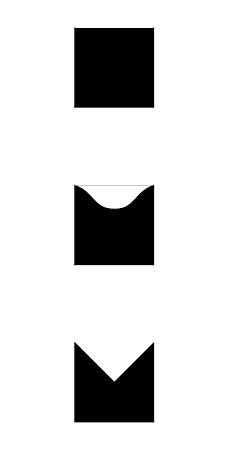
\begin{tikzpicture}
		\fill[\shadinga] (0,2)--(0,3)--(1,3)--(1,2)--(0,2);
		\draw (0,2)--(0,3)--(1,2)--(1,3)--(0,2)--(1,2);
		\draw (0,3) -- (1,3);
		\fill[\shadinga] (0,0)--(0,1)--(1,1)--(1,0)--(0,0);
		\draw[fill=white] plot[smooth ,  tension =1] coordinates {(-0.4,1)(0,1)(0.5,0.7)(1,1)(1.4,1)};
		\fill[white] (-0.6,1) -- (-0.4,0.8) -- (0.4,1.2) -- (0.6,1.2) -- (1.4,0.8) -- (1.6,1) -- (0.6,1.4) -- cycle;
		\draw (0,0)--(0,1)--(1,0)--(1,1)--(0,0)--(1,0);
\draw[fill=\shadinga] (0,-1) -- (0,-2) -- (1,-2) -- (1,-1) -- (0.5,-1.5) -- cycle;
\draw (0,-2) -- (0.5,-1.5) -- (1,-2);
\end{tikzpicture}}

While simplicial collapse is a new operation, one might think of it as the successor to the contraction and subdivision operations we looked at in Section \ref{sec:graph:Minors}. 

\begin{definition}
We say that $X$ is contractible if it simplicially collapses to a point. We say that $X, Y$ are \emph{simplicially homotopic} if they have a common simplicial collapse. 
\end{definition}
We've looked at many contractible space, and we have already developed some notation from Morse theory to represent a sequence of simplicial collapses. Simplicial collapse plays well with the ideas from Discrete morse theory,\project  and prescribe how one can convert descriptions of spaces by simplicial complexes into descriptions by CW-complexes. 

\examplefigure{Let $X= (\Delta, \mathcal S)$ be a triangulated planar surface \emph{excluding} its exterior face. 	Then $X$ is contractible by applications of contractions on it's exterior edges, and then contracting the resulting tree. We will often represent such a series of simplicial collapses by using a diagram of arrows showing the direction of the collapses. }{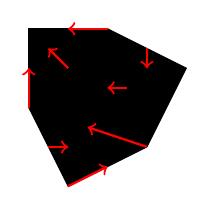
\begin{tikzpicture}[scale=.5]
\draw[fill=\shadinga] (-2.5,0.5) -- (-2.5,-1.5) -- (-1.5,-3.5) -- (0.5,-2.5) -- (1.5,-0.5) -- (-0.5,0.5) -- cycle;
\draw (-0.5,0.5) -- (-2.5,-1.5);
\draw (0.5,-2.5) -- (-2.5,-1.5);
\draw (0.5,-2.5) -- (-0.5,0.5);
\draw[->, red, thick] (-1.5,-0.5) -- (-2,0);
\draw[->, red, thick] (0,-1) -- (-0.5,-1);
\draw[->, red, thick] (-2,-2.5) -- (-1.5,-2.5);
\draw[->, red, thick] (0.5,0) -- (0.5,-0.5);
\draw[->, red, thick] (-1.5,-3.5) -- (-0.5,-3);
\draw[->, red, thick] (0.5,-2.5) -- (-1,-2);
\draw[->, red, thick] (-0.5,0.5) -- (-1.5,0.5);
\draw[->, red, thick] (-2.5,-1.5) -- (-2.5,-0.5);
\end{tikzpicture}}
Between $X_{\tau\to\sigma}\to X$ there is an obvious inclusion. We would like to show that this map induces an isomorphism on the homology. 

\begin{theorem}
Let $Y=X_{\tau\to \sigma}$. Then the map $i: Y\to X$ induces an isomorphism on the homology groups 
\[i:H_k(Y)\xrightarrow{\sim}  H_k(X).\] 
\end{theorem}
\begin{proof}
To prove this theorem, we show that $i$ is a \emph{quasi-isomorphism} in the sense of Definition \ref{def:quasiisomorphism}. This means that we'll need to construct a map $\pi: C_k(X)\to C_k(Y)$ so the compositions 
\[ \pi \circ i: C_k(Y)\to C_k(Y) \;\;\;\; i\circ \pi: C_k(X)\to C_k(X)\]
are both identity on homology. In this case, we are explicitly giving a \emph{quasi-inverse} to $i$. \\
The proposed map $\pi: C_k(X)\to C_k(Y)$ is defined on the basis of simplices by 
\[\pi(\rho)=\left\{ \begin{array}{ll} \rho & \rho \neq \sigma, \tau\\ \partial(\sigma)-\tau & \rho = \tau \\
0 & \rho = \sigma \end{array} \right. .\]
Geometrically, this map sends the collapsed simplex to 0, and the collapsing facet to the other facets it was pushed into. See Figure \ref{fig:collapsinghomotopy} for an intuition of this construction. 
\begin{figure}
\centering
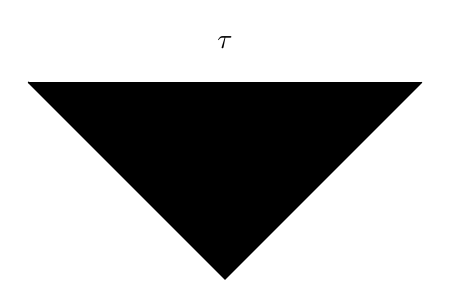
\begin{tikzpicture}
\draw[fill=\shadinga] (-3.5,3) -- (-1,0.5) -- (1.5,3);
\draw[->]  plot[smooth, tension=.7] coordinates {(-1.5,3) (-1.5,2) (-2,1.5)};
\draw[->]  plot[smooth, tension=.7] coordinates {(-0.5,3) (-0.5,2) (0,1.5)};
\draw[dashed] (-3.5,3) -- (1.5,3);
\draw[dotted]  plot[smooth, tension=.7] coordinates {(-3.5,3) (-2,2.5) (-1,2) (0,2.5) (1.5,3)};
\draw[dotted]  plot[smooth, tension=.7] coordinates {(-3.5,3) (-1.5,1.5) (-1,1) (-0.5,1.5) (0,2) (1.5,3)};
\node at (-1,1.5) {$\sigma$};
\node at (-1,3.5) {$\tau$};
\end{tikzpicture}
\caption{Deforming through a face as a homotopy}
\label{fig:collapsinghomotopy}
\end{figure}
\begin{lemma}
The compositions \[ \pi \circ i: C_k(Y)\to C_k(Y) \;\;\;\; i\circ \pi: C_k(X)\to C_k(X)\] are both chain homotopic to the identity. 
\end{lemma}
For $\pi \circ i: C_k(Y)\to C_k(Y)$, we don't need to do anything, as this is honestly the identity on the chain complex. \\
For the composition $i\circ \pi: C_k(X)\to C_k(X)$, we check that on a simplex, 
\[i\circ \pi(\rho)=\left\{ \begin{array}{ll} \rho & \rho \neq \sigma, \tau\\ \partial(\sigma)-\tau & \rho = \tau \\
0 & \rho = \sigma \end{array} \right. .\]
We would like to propose a homotopy $h_k: C_k(Y)\to C_{k+1}(Y)$ which ``deforms'' out the difference between this map and the identity. So, we would like to find a homotopy $h_k:C_k(Y)\to C_{k+1}(Y)$ so that $\partial^Yh+h\partial^Y$ gives the difference 
\[(i\circ \pi-\id)(\rho)=\left\{ \begin{array}{ll} 0 & \rho \neq \sigma, \tau\\ \partial(\sigma) & \rho = \tau \\
\sigma & \rho = \sigma \end{array} \right. \]
A candidate homotopy is inspired by  our picture: notice that there is a correspondence between $\tau$ and the 1-dimensional higher $\sigma$. It would make sense to have 
\[h(\rho) = \left\{ \begin{array}{ll} 0 & \rho \neq \tau \\ \sigma & \rho = \tau \end{array}\right. 
\]
This turns out to give us our chain homotopy. Let's look at what the composition $\partial h + h \partial$ is in the three cases we looked at above. 
\begin{itemize}
\item If $\rho\neq \tau, \sigma$, then $(\partial h + h \partial)(\rho)=0.$ This crucially depends on the fact that $\tau, \sigma$ are not subsimplices of $\partial(\rho)$ by our definition of simplicial collapse. 
\item When we apply our composition to $\tau$, we get 
\[(\partial\circ h + h \circ \partial)(\tau) = \partial( \sigma)  + h (\partial \tau) = \partial\sigma= (i\circ \pi-\id)(\tau). \]
\item When we apply our composition to $\sigma$, we similarly get 
\[(\partial\circ h + h \circ \partial)(\sigma) = \partial(0)+ h \partial(\sigma) = \sigma = (i\circ \pi - \id)(\sigma). \]
\end{itemize}
So, we see that $h$ gives a chain homotopy between $(i\circ \pi)$ and the identity. We therefore conclude that the resulting map is the identity on homology, and that $C_\bullet(X)$ and $C_\bullet(Y)$ are quasi-isomorphic. 
\end{proof}
This theorem will allow us to quickly compute the homology of spaces by taking a homotopy equivalences between spaces. For example, we already know the homology of a large class of topological spaces.
\begin{corollary}
If $X$ is contractible, then $H_k(X)=H_k(pt)$. 
\end{corollary}
In theory, we could extend the types of contractions and subdivisions we allow to a larger list, and get more flexible tools for understanding the homology of spaces. In practice, we will be content with this one operation, with the understanding that if one wants to develop more flexible types of deformations between spaces, one should probably upgrade from simplicial complexes to actual point-set topology. Here is such an example. \\

\examplefigure{Let $X=X_1\sqcup X_2\cup \{e\}$ be a simplicial complex made of 3 parts: two simplicial complexes joined by an edge. Then the simplicial complex $X/e=X_1\sqcup X_2$ where the vertices at the ends of $e$ have been ``fused'' together is not a simplicial collapse of the original complex. Despite this, the intution that $C_\bullet(X)$ is homotopy equivalent to $C_\bullet(X/e)$ is correct.}
{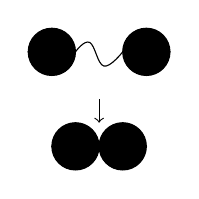
\begin{tikzpicture}[scale=.3]
\draw[fill=\shadinga]  (1,-4)  {} ellipse (1 and 1);
\draw   (1,-4)  ellipse (1 and .2);
\draw[fill=\shadinga]  (4,0)  {} ellipse (1 and 1);
\draw   (4,0)  ellipse (1 and .2);
\draw[fill=\shadinga]  (3,-4)  {} ellipse (1 and 1);
\draw   (3,-4)  ellipse (1 and .2);
\draw[fill=\shadinga]  (0,0)  {} ellipse (1 and 1);
\draw   (0,0)  ellipse (1 and .2);
\draw  plot[smooth, tension=.7] coordinates {(1,0) (1.6,0.4) (2.2,-0.6) (3,0)};
\draw[->] (2,-2) -- (2,-3);
\end{tikzpicture}}
An intermediate step between abstract simplicial complexes and full topological spaces are \emph{CW complexes}. In a CW complex, you still glue disks together along their boundaries,\project but you allow the gluings to be continuous, instead of rigidly along subsimplices. Associated to a CW complex is the \emph{CW-chain complex}, whose differential is defined with a little more difficulty.

\label{sec:simplicialmaps}

		


\section{Exercises}


\begin{exercise}\label{exer:simp:homtorus}
Give a triangulation of the Torus, and compute its homology.
\end{exercise}

\begin{exercise}\label{exer:simp:homklein}
Give a triangulation of the Klein bottle, and compute its homology. 
\end{exercise}

\begin{exercise}\label{exer:simp:spherebyhand}
Prove by hand that the homology of the sphere $H_k(S^n)$ is zero whenever $n\neq k, 0$. 
\end{exercise}

\begin{exercise}\label{exer:simp:homologystronger}
Construct two simplicial complexes $X$ and $Y$ which have the same Euler characteristic, but different homology groups. (This proves that homology is a stronger tool to study topological spaces than Euler Characteristic, as whenever $X$ and $Y$ have the same homology groups, they have the same Euler Characteristic.)
\end{exercise}

\begin{exercise}\label{exer:simp:arbitraryhom}
Let $b_0, \ldots, b_n$ be an arbitrary sequence. Construct a simplicial complex $X$ with $\dim(H_k(X))=b_k$. 
\end{exercise}



\begin{exercise}
\label{exer:homsphere}
Using induction, show that $H^n(S^n)=\Z_2$ by using the \ref{cor:coneles} and \ref{exam:conesphere}.
\end{exercise}

\begin{exercise}\label{exer:hom:conecontract}
Show that for every $X$, there exists a space $Y$ and an injective simplicial map $i: X\to Y$ so that $H_k(Y)=0$ for all $k\geq 1$. 
\end{exercise}

One of the main uses of $\cone$ is to create new topological spaces. Let $x$ be the topological space consisting of a single point. A topological space is an \emph{iterated cone} if it can be created from written as a sequence of mapping cones and disjoint unions of points. For example, one may make a triangle by taking the iterated mapping cone:
\[\cone(i:x\cup x \to  \cone(\id:x\to x)).\]
where the map $i:x\cup x\to \cone(\id(x\to x))$ is inclusion to the left and right endpoints. 
\begin{exercise}\label{exer:hom:iteratedmapping}
Show that all disks and all spheres can be constructed as iterated mapping cones. 
\end{exercise}

\begin{exercise}\label{exer:hom:graphiterated}
 Show that every graph is a topological minor of an interated cone. 
\end{exercise}

\begin{exercise}\label{exer:hom:coneedge}
Let $X$ be a connected simplicial complex, $v, w$ two vertices of the simplicial complex so that $vw$ is not an edge in $X$. Show that the simplicial complex $X\cup \{e\}$, where $e$ as a new edge between $vw$ has $H_1(X\cup\{e\})=H_1(X)\oplus \Z$, and $H_k(X\cup\{e\})=H_k(X)$ when $k\neq 1$. 
\end{exercise}

Let $X$ be a simplicial complex. The \emph{suspension} of $X$ is the simplicial complex given by successively taking two cones:
\[\Sigma X=\cone(i:X\to \cone(\id:X\to X)).\]
The $n$-fold suspension is given by $\Sigma^kX:=\underbrace{\Sigma\cdot \Sigma}_{k \text{ times}} X$. 
\begin{exercise}\label{exer:hom:suspensioneuler}
Compute the Euler characteristic of $\Sigma X$ in terms of the Euler characteristic of $X$. 
\end{exercise}

\begin{exercise}\label{exer:hom:suspension}
Let $S^0=\{x, y\}$ be the two point space. Draw out the  $k=0, 1, 2$ the spaces
\[\Sigma^k S^0.\]
Make a geometric argument for why these spaces are topologically spheres, and then compute $H^k(\Sigma^k S^0).$ 
\end{exercise}

\begin{exercise}\label{exer:hom:suspensionhomology}
Show that whenever $k\geq 1$, 
\[H_{k+1}(\Sigma X ) = H_k(X). \]
\end{exercise}






\begin{exercise}
Two chain complexes are \emph{quasi-isomorphic} if there exists a chain map $f: A_\bullet\to B_\bullet$ so that $f_*: H_\bullet(A)\to H_\bullet(B)$ is an isomorphism. Find two chain complexes $A_\bullet, B_\bullet$ so that their homologies are isomorphic, but $A_\bullet, B_\bullet$ are \emph{not} quasiisomorphic. (You will have to work with modules.)
\end{exercise}

\begin{exercise}
Let $X$ be a simplicial complex, and $\sigma$ a simplex of $X$. Pick $\tau \subset \sigma$ a subsimplex. Suppose $x$ is a vertex so that whenever $x\in \tau$, we have that $\tau\subset \sigma$.  We define the simplicial complex $X\setminus x$ to be the simplicial complex with all the simplices of $X$ except those which include the vertex $x$. Show that $H_k(X\setminus x)=H_k(X)$. 
\end{exercise}

\begin{exercise}
Let $X$ be a simplicial complex, and suppose that there is a morse function $f: X\to \R$ which has only 1 critical point. Show that the homology of $X$ is that of a point. 
\end{exercise}

\begin{exercise}
Suppose that $X$ is a simplicial complex which is a graph. Show that it is contractible if and only if it is a tree. 
\end{exercise}


\begin{exercise}
What is the structure of $\Delta(\overline {P(\Delta)})$?
\end{exercise}

\begin{exercise}
Show that $\Delta(\overline{P(\Delta)})$ is homotopic to $\Delta(\overline{P(\Delta)})$.  
\end{exercise}